%!TEX root = ./template-skripsi.tex
%-------------------------------------------------------------------------------
%                            BAB III
%               			PEMBAHASAN
%-------------------------------------------------------------------------------

\chapter{METODOLOGI PENELITIAN}


\section {Deskripsi Penelitian}

Pada penelitian ini akan merancang tampilan dan aplikasi \textit{web} dengan \textit{admin console} untuk \textit{search engine} yang telah dibuat pada penelitian sebelumnya. Berikut merupakan tahapan-tahapan penelitian yang penulis akan lakukan dalam perancangan aplikasi:


\begin{figure}[H]
	\centering
	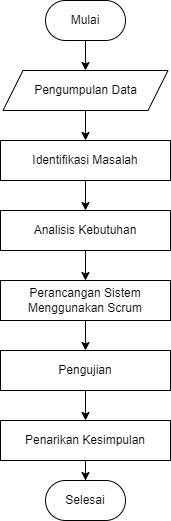
\includegraphics[keepaspectratio, width=3cm]{gambar/flowchart.png}
	\caption{Tahapan penelitian}
	\label{gambar:flowchart.png}
\end{figure}


\section {Pengumpulan Data}

Peneliti melakukan studi literatur dengan membaca jurnal-jurnal, penelitian terdahulu dan buku yang berkaitan dengan topik penelitian.

\section {Analisa Kebutuhan Sistem}

Dalam penelitian ini, beberapa perangkat keras yang digunakan untuk menunjang pembuatan sistem adalah sebagai berikut:

\begin{enumerate}
	\item Laptop yang mempunyai CPU Intel Core i5-8250U 1.60 GHz (8 Cores) dengan RAM sebesar 12 GB
	\item Koneksi berbasis Wi-Fi
\end{enumerate}

Perangkat keras yang telah disebutkan sudah memenuhi persyaratan dalam menjalankan perangkat lunak yang akan digunakan seperti:

\begin{enumerate}
	\item Windows 10 64 bit
	\item Visual Studio Code
	\item Figma
	\item Adobe Illustrator CC6
\end{enumerate}

\section {Perancangan Sistem Dengan Scrum}


%Dalam penelitian ini akan digunakan metode \textit{scrum} agar penelitian ini menjadi lebih terstruktur dan mudah. Desain penelitian akan menjelaskan tahapan tahapan yang akan dilakukan penulis dalam penelitian ini dengan menggunakan metode \textit{scrum}.
%
%\begin{figure}[H]
%	\centering
%	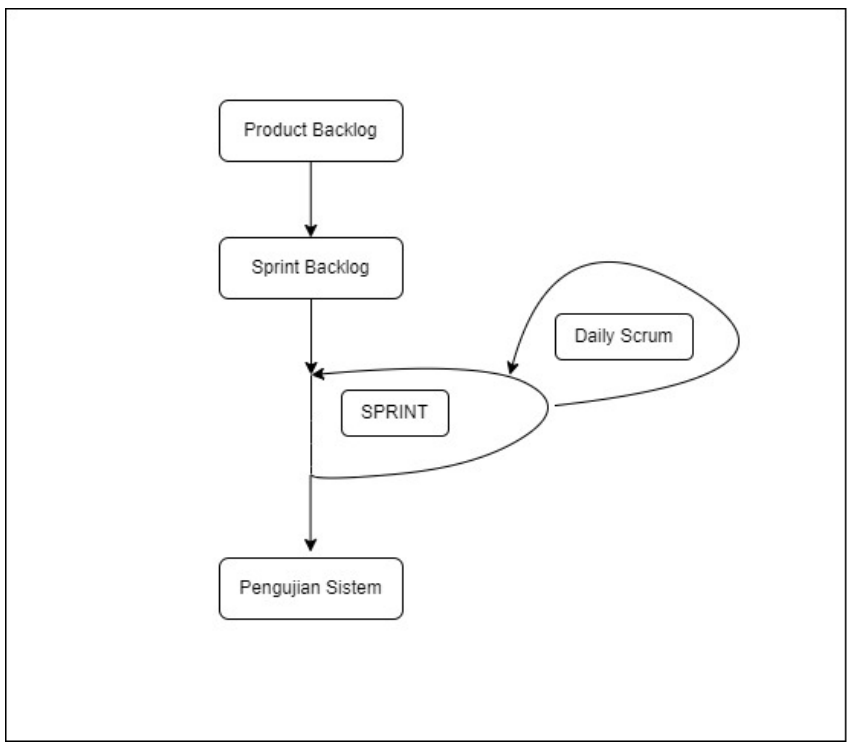
\includegraphics[keepaspectratio, width=13cm]{gambar/desain-penelitianpng.png}
%	\caption{Desain Penelitian}
%	\label{gambar:desain-penelitianpng.png}
%\end{figure}

%Tahap pertama yang akan dilakukan pada penelitian ini adalah membuat \textit{product backlog} dari sistem yang akan dibuat, lalu membuat jadwal pengerjaan atau \textit{sprint backlog}. Setelah itu, sprint dimulai dengan diselingi \textit{daily scrum} untuk melaporkan progress dan menentukan task selanjutnya. Setelah sistem selesai dikerjakan di dalam sprint, maka dilakukan pengujian sistem.

Agar penelitian ini menjadi lebih terstruktur dan mudah, maka penelitian ini akan menggunakan metode \textit{scrum} sebagai metode pengembangan sistemnya. Berdasarkan gambar \ref{gambar:desain-penelitianpng.png}, komponen-komponen \textit{scrum} terdiri dari \textit{product backlog}, \textit{sprint backlog}, \textit{daily scrum} dan \textit{sprint} lalu dilanjutkan dengan pengujian sistem yang sudah dibuat.


\begin{figure}[H]
	\centering
	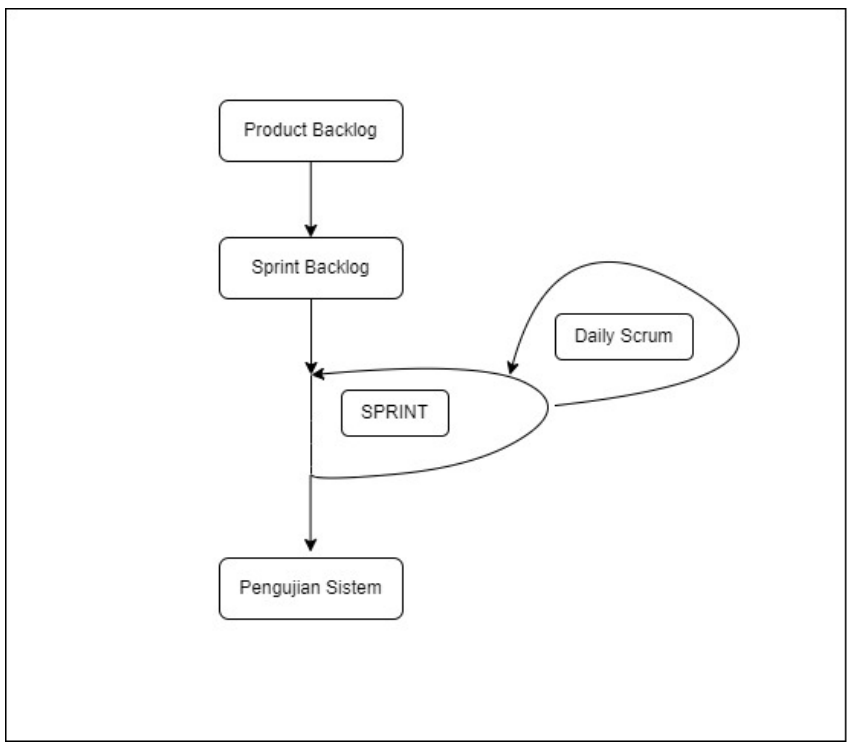
\includegraphics[keepaspectratio, width=13cm]{gambar/desain-penelitianpng.png}
	\caption{Tahapan penelitian dengan menggunakan metode \textit{scrum}}
	\label{gambar:desain-penelitianpng.png}
\end{figure}

\begin{enumerate}
	\item \textit{Product backlog}

	\textit{Product backlog} merupakan kumpulan tugas yang akan dilaksanakan. \textit{Product backlog} seperti ditunjukan oleh tabel \ref{productbacklog} penelitian ini terdiri dari 3 komponen yaitu \textit{story}, \textit{sprint} dan \textit{status}. \textit{Story} ialah sebuah pekerjaan besar yang dapat dibagi bagi lebih kecil lagi menjadi tugas tugas kecil. \textit{Sprint} menandakan \textit{sprint} berapa \textit{story} tersebut akan diselesaikan. \textit{Status} memberitahu apakah \textit{sprint} tersebut sudah terlaksanakan atau belum.
	
	\begin{table}[H]
		\centering
		\caption{\textit{Product Backlog}}
		\label{productbacklog}
		\begin{tabular}{@{} |p{1cm}|p{7cm}| p{1cm} |p{2.5cm}|@{}}
			\hline
			\textbf{No.} & \textbf{\textit{Story}} & \textbf{\textit{Sprint}} & \textbf{\textit{Status}} \\
			\hline
			1 & Fitur pencarian pengguna & 1, 2, 8 & Selesai \\
			\hline
			2 & Fitur \textit{page ranking} & 4, 5 & Selesai\\
			\hline
			3 & Fitur \textit{staff} & 5, 8 & Selesai\\
			\hline
			4 & Fitur \textit{document ranking} & 5, 7  & Selesai\\
			\hline
			5 & Fitur \textit{crawling} & 3, 6 & Selesai\\
			\hline
			6 & Struktur projek & 2 & Selesai\\
			\hline
			7 & \textit{multi-threaded service} & 10  & Selesai\\
			\hline
			8 & \textit{Service deployment} & 11  & Selesai\\
			\hline
			9 & Background task dengan \textit{Celery} & 12  & Selesai\\
			\hline
			10 & Pengujian penggunaan memori & 13  & Selesai\\
			\hline
		\end{tabular}
	\end{table}

	\item{Sprint Backlog}
	
	\textit{Sprint backlog} merupakan daftar tugas tugas kecil yang perlu dilaksanakan pada suatu \textit{sprint}.
	
	\item{Sprint}
	
	\textit{Sprint} merupakan masa dimana pengerjaan tugas tugas yang telah direncanakan pada suatu \textit{sprint} dilakukan. Lama durasi setiap \textit{sprint} ditentukan oleh \textit{scrum master} yang telah disepakati bersama.
	
	\item{Daily Scrum}
	
	\textit{Daily scrum} merupakan pertemuan dengan \textit{scrum master} untuk membahas tugas apa yang telah dicapai hari kemarin dan tugas apa yang ingin dicapai hari ini yang dilaksanakan setiap hari.
\end{enumerate}

% Tahapan pertama yang dilakukan pada penelitian ini adalah mendefinisikan sebuah \textit{product backlog} penelitian dan mendifinisikan \textit{sprint backlog} yang merupakan jadwal pengerjaan tugas tugas yang akan dibuat. Setelah kedua komponen tersebut berhasil dibuat, maka \textit{sprint} dapat dimulai dari awal dengan diselingi \textit{daily scrum} untuk melakukan pelaporan \textit{progress} penelitian yang sedang dilakukan. Berikut ini adalah tabel \textit{product backlog} yang telah dibuat. 


%
%
%Berdasarkan tabel \ref{productbacklog}, \textit{product backlog} penelitian ini terdiri dari 3 komponen yaitu \textit{story}, \textit{sprint} dan \textit{status}. \textit{Story} ialah sebuah pekerjaan besar yang dapat dibagi bagi lebih kecil lagi menjadi tugas tugas kecil. \textit{Sprint} menandakan \textit{sprint} berapa \textit{story} tersebut akan diselesaikan. \textit{Status} memberitahu apakah \textit{sprint} tersebut sudah terlaksanakan atau belum.
%
%\section{\textit{Sprint} 1}
%
%\begin{table}[H]
%	\centering
%	\caption{\textit{Sprint-1 Backlog}}
%	\label{uat}
%	\begin{tabular}{@{} |p{1cm}|p{3cm}| p{6cm} |p{2.5cm}|@{}}
	%		\hline
	%		\textbf{No.} & \textbf{\textit{Story}} & \textbf{\textit{Task}} & \textbf{\textit{Status}} \\
	%		\hline
	%		1 & Membuat rancangan tampilan dashboard \textit{search engine} & \begin{enumerate}
		%			\item Penentuan desain sistem
		%			\item Perancangan desain halaman kelola admin
		%			\item Perancangan desain halaman \textit{page rank matrix}
		%			\item Perancangan desain halaman peta situs admin
		%			\item Perancangan desain halaman pencarian pengguna
		%			\item Perancangan desain halaman peta situs pengguna
		%			\item Perancangan desain halaman hasil pencarian pengguna
		%			\item Perancangan desain halaman ranking situs			
		%			\item Pendataan route table yang sudah ada dengan tampilan yang ada
		%			\item Desain route table untuk web service yang belum ada
		%		\end{enumerate} & \\
	%		\hline
	%		
	%	\end{tabular}
%\end{table}
%Pada \textit{sprint} ini akan dilakukan perancangan tampilan untuk \textit{search engine} ONE (\textit{Omniscience Network Extractor}) dilakukan dengan perangkat lunak Figma dan Adobe Illustrator. Untuk memudahkan proses dalam perancangan tampilan untuk \textit{search engine} yang akan dibangun, diperlukan adanya suatu sistem desain untuk \textit{sizing}, \textit{spacing} dan \textit{color} atau warna.
%
%Dalam sistem desain untuk \textit{spacing} dan \textit{sizing} digunakan seperti tabel berikut
%
%\begin{table}[H]
%	\caption{\textit{Sistem desain \textit{sizing} dan \textit{spacing}}}
%	\label{Sistem desain sizing dan spacing}
%	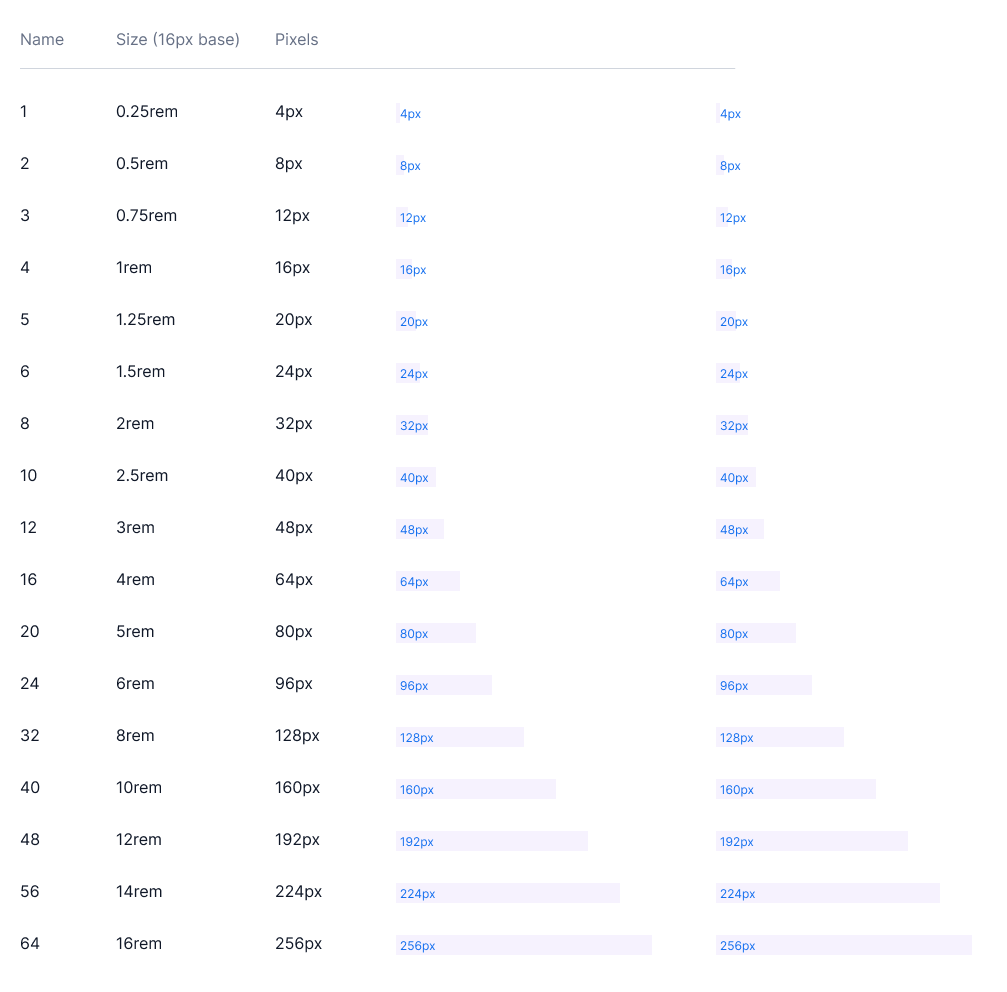
\includegraphics[keepaspectratio, width=13cm]{gambar/g-109.png}
%\end{table}
%
%Untuk sistem desain warna, warna biru \textit{navy} digunakan sebagai warna utama tampilan \textit{search engine}. Adapun \textit{shades} dari warna utama yaitu \textit{navy} adalah sebagai berikut. Warna \textit{shades} ditentukan dengan cara mengatur nilai \textit{hue}, \textit{saturation} dan \textit{lightning} dari warna utama.
%
%
%\begin{figure}[H]
%	\centering
%	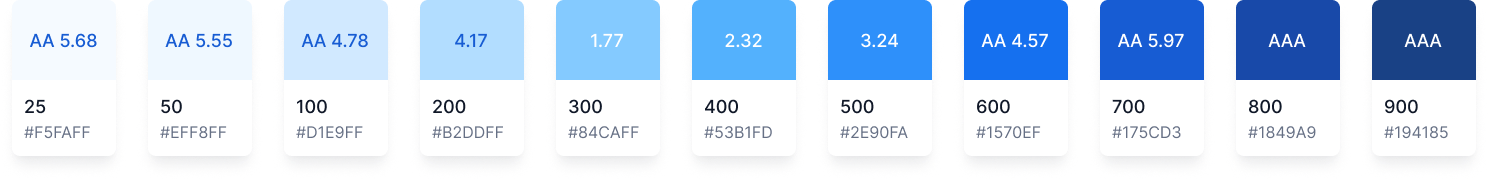
\includegraphics[keepaspectratio, width=13cm]{gambar/g-110.png}
%	\caption{Desain Penelitian}
%	\label{gambar:g-110.png}
%\end{figure}
%
%Hal pertama yang dilakukan dalam pembuatan tampilan dari \textit{search engine} adalah mendesain sebuah logo. Sebuah logo digunakan sebagai identitas bagi \textit{search engine} yang akan dibuat tentulah harus mempunyai makna. Logo yang akan dibuat berbentuk "O" melambangkan huruf pertama dari nama search engine tersebut yaitu "ONE". Tanpa warna, logo pola jaring akan terlihat dalam lingkaran berbentuk O yang melambangkan suatu hubungan dari banyaknya sebuah situs. Untuk pewarnaan, digunakan warna oranye yang melambangkan huruf O dari nama \textit{search engine} tersebut, warna \textit{navy} melambangkan huruf N dari nama \textit{search engine} dan warna \textit{eclipse} melambangkan huruf terakhir dari \textit{search engine} tersebut yaitu E.
%
%
%\begin{figure}[H]
%	\centering
%	
\includegraphics[keepaspectratio, width=13cm]{gambar/g-111.png}
%	\caption{Desain Logo ONE \textit{Search Engine}}
%	\label{gambar:g-111.png}
%\end{figure}
%
%\begin{figure}[H]
%	\centering
%	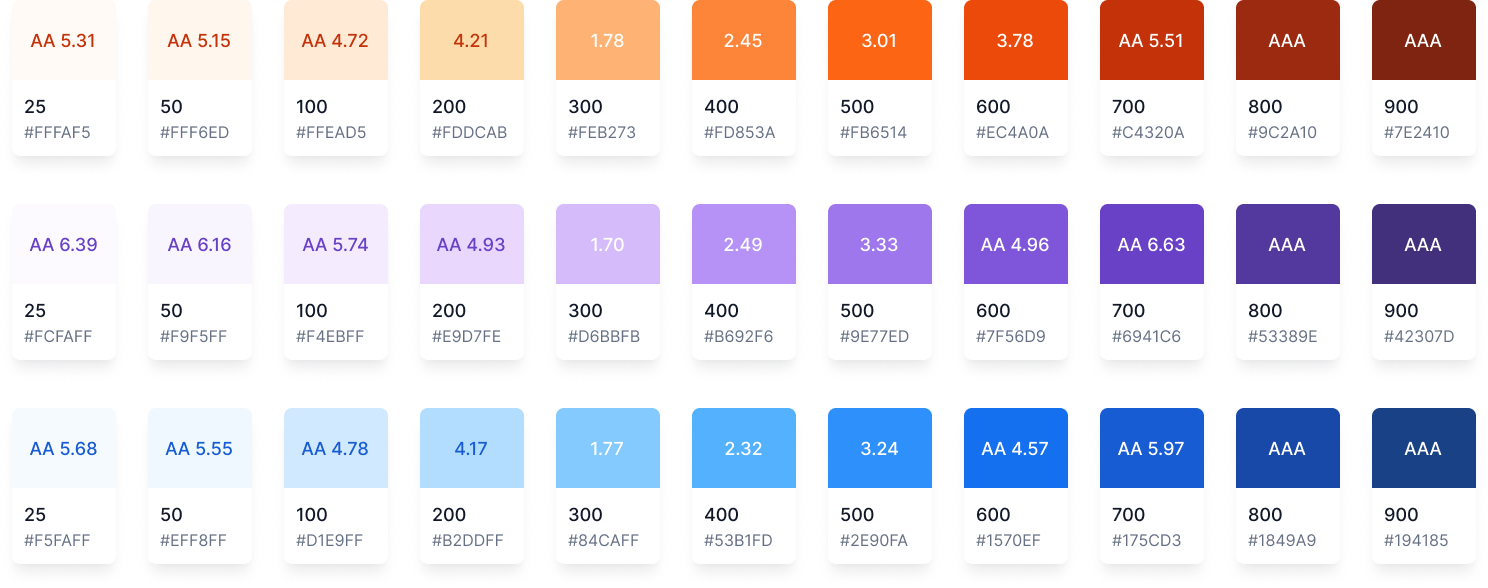
\includegraphics[keepaspectratio, width=13cm]{gambar/g-113.png}
%	\caption{Desain sistem warna pada logo ONE}
%	\label{gambar:g-113.png}
%\end{figure}
%%
%%Penelitian ini akan menggunakan data yang berasal dari penelitian \citep{lazu} yang digunakan berasal dari proses \textit{crawling} yang dilakukan sebelumnya. Pada penelitian \citep{lazu} telah dibuat aplikasi berbasis flask untuk menyediakan cara yang mudah bagi tampilan aplikasi untuk berkomunikasi dengan data yang telah disediakan. Untuk menghubungkan data dari penelitian yang telah disediakan dengan tampilan yang akan dibuat digunakan sebuah \textit{Application Programming Interface} yang memenuhi arsitektur desain perangkat lunak {Representational State Transfer} atau biasa disebut dengan \textit{Rest API}. Adapun skema {Rest API} yang telah dibuat oleh \citep{lazu} adalah sebagai berikut.
%%
%%\begin{table}[H]
%%	\caption{\textit{Routing table REST API}}
%%	\label{routing_table}
%%	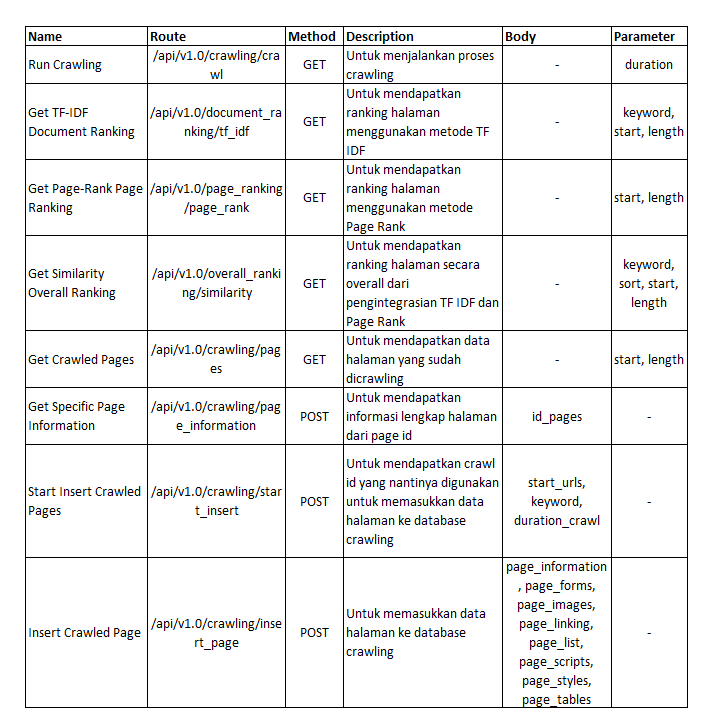
\includegraphics[keepaspectratio, width=13cm]{gambar/routing_table}
%%\end{table}
%%
%%Terdapat tambahan \textit{Routing} guna untuk memenuhi fitur yang akan dibangun yaitu
%%
%%
%%\begin{table}[H]
%%	\centering
%%	\caption{\textit{Routing Table Tambahan}}
%%	\label{uat}
%%	\begin{tabular}{@{} |p{1cm}|p{5cm}| p{2cm}|p{2cm}|p{2cm}|p{2cm} |p{2cm}|@{}}
	%%		\hline
	%%		\textbf{Name} & \textbf{\textit{Route}} & \textbf{\textit{Method}} & \textbf{\textit{Description}}  & \textbf{\textit{Body}} & \textbf{\textit{Query}} \\
	%%		\hline
	%%		1 & /api/v1/domains & GET & Mendapatkan daftar domain yang berhasil di crawl & - & page, limit, countries, query \\
	%%		\hline
	%%		2 & /api/v1/metrics & GET & Mendapatkan statistik \textit{crawler} &   & - \\
	%%		\hline
	%%		3 & /api/v1/admins & GET & Mendapatkan daftar admin \textit{crawler} & -  &  page, limit, roles, query \\
	%%		\hline
	%%		4 & /api/v1/admins/:id/delete & DELETE & Menghapus admin & -  &  - \\
	%%		\hline
	%%		5 & /api/v1/admins/:id/update & PATCH & Mengupdate admin & firstName, lastName, username, role, status, email, profilePictureUrl  &  - \\
	%%		\hline
	%%		6 & /api/v1/admins/:id & GET & Mendapatkan data admin & - &  - \\
	%%		\hline
	%%		7  & /api/v1/login & POST & Login admin & - & - \\
	%%		\hline
	%%	\end{tabular}
%%\end{table}
%%
%%
%%Dari tabel \textit{REST API} diatas dan analisa database yang telah dilakukan sebelumnya, akan dilakukan pembuatan desain tampilan untuk \textit{search engine}. 
%
%Terdapat dua bagian dari tampilan \textit{search engine}, yaitu bagian untuk admin untuk manajemen \textit{search engine} dan tampilan untuk \textit{pengguna}.
%
%\subsection{Penentuan \textit{Font}}
%
%Menurut \citep{refactoringui}, jenis font dapat ditentukan dengan observasi jenis \textit{font} yang digunakan dari aplikasi lain yang sudah ada di pasaran. Pada dasarnya, aplikasi yang sudah ada di pasasran memiliki beberapa orang perancang yang memiliki pengalaman lebih mengenai \textit{typography} untuk menentukan jenis \textit{font} yang akan mereka gunakan biasanya dengan telah memperhitungkan berbagai faktor. Setelah melakukan observasi pada aplikasi besar yang ada pada pasaran, peneliti memutuskan untuk menggunakan \textit{font} \textit{Inter} sebagai jenis \textit{font} utama pada aplikasi dikarenakan jenis \textit{font} ini sudah banyak sekali digunakan pada aplikasi besar yang terdapat di pasaran dan bersifat \textit{open source}.
%
%\subsection{Penentuan \textit{White Spacing} Komponen}
%
%Dalam penentuan \textit{white spacing} dari setiap komponen yang akan dibuat, penulis menggunakan metode \textit{decremental} seperti yang telah dibahas sebelumnya. Pemberian \textit{white spacing} secara \textit{decremental} adalah sebuah cara untuk menemukan nilai \textit{white spacing} yang cocok digunakan pada komponen yang akan dibuat dengan cara memberikan nilai awal \textit{white spacing} yang besar kepada komponen yang akan dibuat dan mengurangi nilai \textit{white spacing}-nya secara bertahap sampai dapat dikatakan cocok. Dalam pemberian \textit{white spacing} penulis menggunakan sistem desain \textit{white spacing} dan \textit{sizing} yang telah ditentukan sebelumnya.
%
%
%\begin{figure}[H]
%	\centering
%	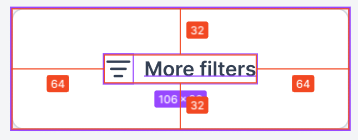
\includegraphics[keepaspectratio, width=13cm]{gambar/example-whitespace-decremental-1.png}
%	\caption{Pemberian nilai \textit{white spacing} awal yang besar terhadap komponen \textit{button}}
%	\label{gambar:example-whitespace-decremental-1.png}
%\end{figure}
%
%
%\begin{figure}[H]
%	\centering
%	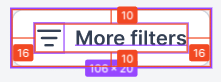
\includegraphics[keepaspectratio, width=13cm]{gambar/example-whitespace-decremental-2.png}
%	\caption{Pemberian nilai \textit{white spacing} secara \textit{decremental} terhadap komponen \textit{button} sehingga \textit{white spacing} yang diberikan terasa cocok}
%	\label{gambar:example-whitespace-decremental-2.png}
%\end{figure}
%
%
%
%\subsection{Halaman \textit{Dashboard} Admin}
%
%Pada desain halaman dashboard untuk admin yang telah dibuat, terdapat bagian \textit{search engine metrics}. Pada bagian ini terdapat informasi dari \textit{search engine} seperti korelasi \textit{pagerank}, total \textit{assets} yang berhasil di-\textit{crawl}, statistik url yang telah di-\textit{crawl}, total jumlah url yang telah di-\textit{crawl} dan jumlah kata yang telah di-\textit{crawl}. Pada halaman ini juga terdapat tabel yang dapat digunakan untuk mengelola semua url yang telah di-\textit{crawl}. Pada halaman ini jarak antara komponen dalam halaman dibuat lebih kecil guna untuk memuat informasi dalam jumlah banyak dalam satu halaman \citep{refactoringui}. Pada tombol ini terdapat tombol pagerank matrix yang berguna untuk menavigasi admin ke halaman \textit{pagerank matrix}.
%
%\begin{figure}[H]
%	\centering
% 	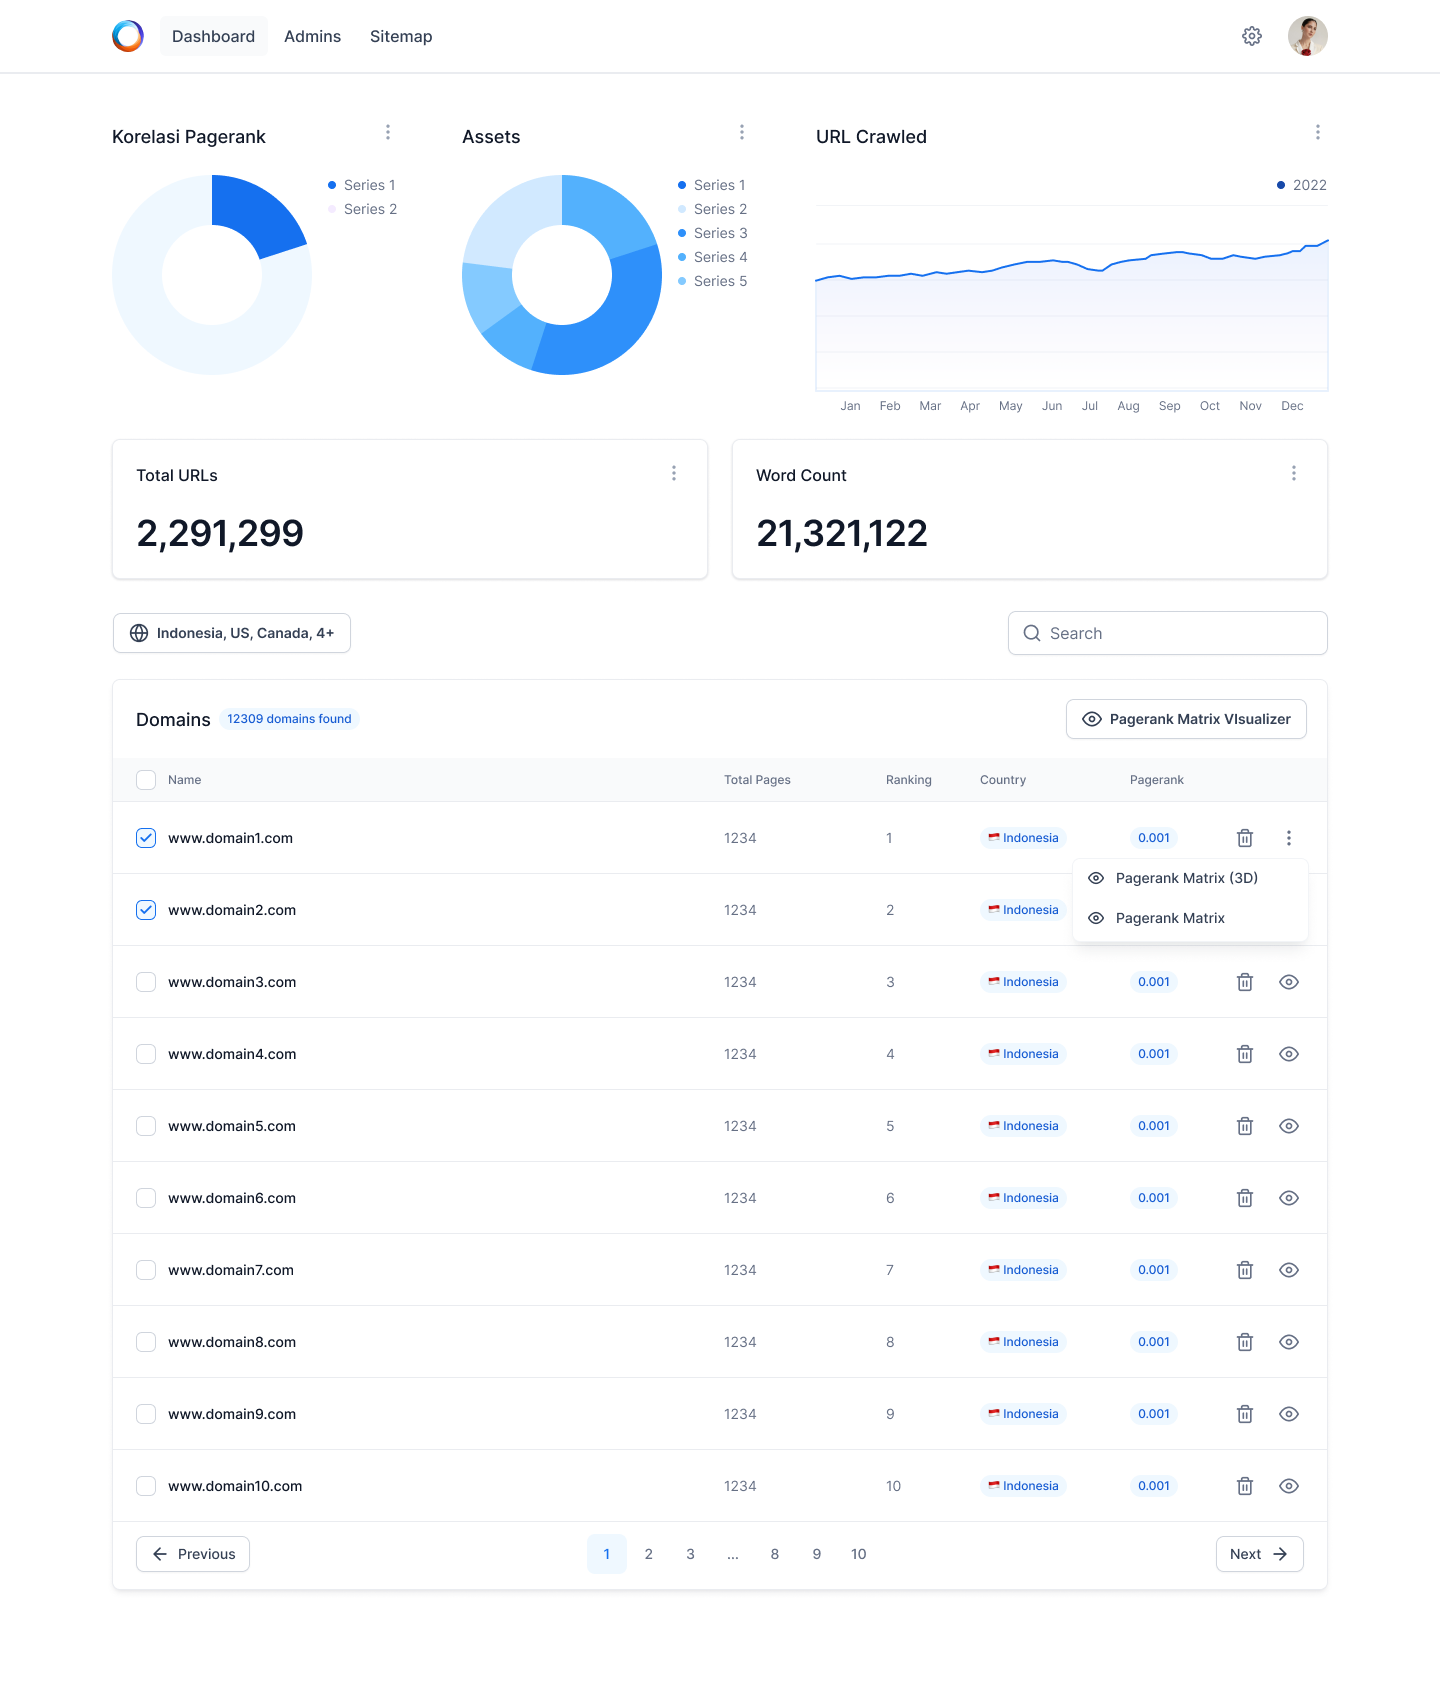
\includegraphics[keepaspectratio, width=13cm]{gambar/g-114.png}
%	\caption{Desain tampilan dashboard \textit{search engine}}
%	\label{gambar:dashboard.png}
%\end{figure}
%
%Adapun routing tabel dari halaman ini adalah sebagai berikut
%
%
%\begin{table}[H]
%	\centering
%	\caption{\textit{Routing Table Halaman Dashboard Admin}}
%	\label{uat}
%	\begin{tabular}{@{} |p{0.5cm}|p{3.5cm}| p{1.5cm}|p{2cm}|p{2cm}|p{2cm} |p{2cm}|p{0.5cm}|@{}}
	%		\hline
	%		\textbf{No.} & \textbf{\textit{Route}} & \textbf{\textit{Method}} & \textbf{\textit{Description}}  & \textbf{\textit{Body}} & \textbf{\textit{Query}} &  \textbf{\textit{Return}} \\
	%		\hline
	%		1 & /api/v1/domains & GET & Mendapatkan daftar domain yang berhasil di crawl & - & page, limit, countries, query & JSON \\
	%		\hline
	%		2 & /api/v1/metrics & GET & Mendapatkan statistik dashboard &   & -  & JSON \\
	%		\hline
	%		3 & /api/v1/domains/:id /delete & DELETE & Menghapus suatu domain & - & - & JSON \\
	%		\hline
	%		4 & /dashboard & GET & Menampilkan halaman dashboard & - & -  & View \\
	%		\hline
	%	\end{tabular}
%\end{table}
%
%\subsection{Halaman \textit{Page Rank Matrix}}
%
%Pada halaman \textit{page rank matrix} admin dapat melihat nilai \textit{page rank matrix} per-domain atau seluruh domain. Pembuatan halaman ini bertujuan agar memudahkan sisi admin dalam melihat \textit{page rank matrix} dari suatu domain ataupun seluruh domain yang berhasil di-\textit{crawl}. Halaman ini tersedia dalam bentuk tiga dimensi dan dua dimensi. Pembuatan halaman ini dalam graf tiga dimensi bertujuan untuk mempermudah pengguna dalam melihat \textit{domain} yang direpresentasikan dengan titik dan garis yang merepresentasikan \textit{outgoing} link dari setiap domain yang ada.
%
%
%\begin{figure}[H]
%	\centering
%	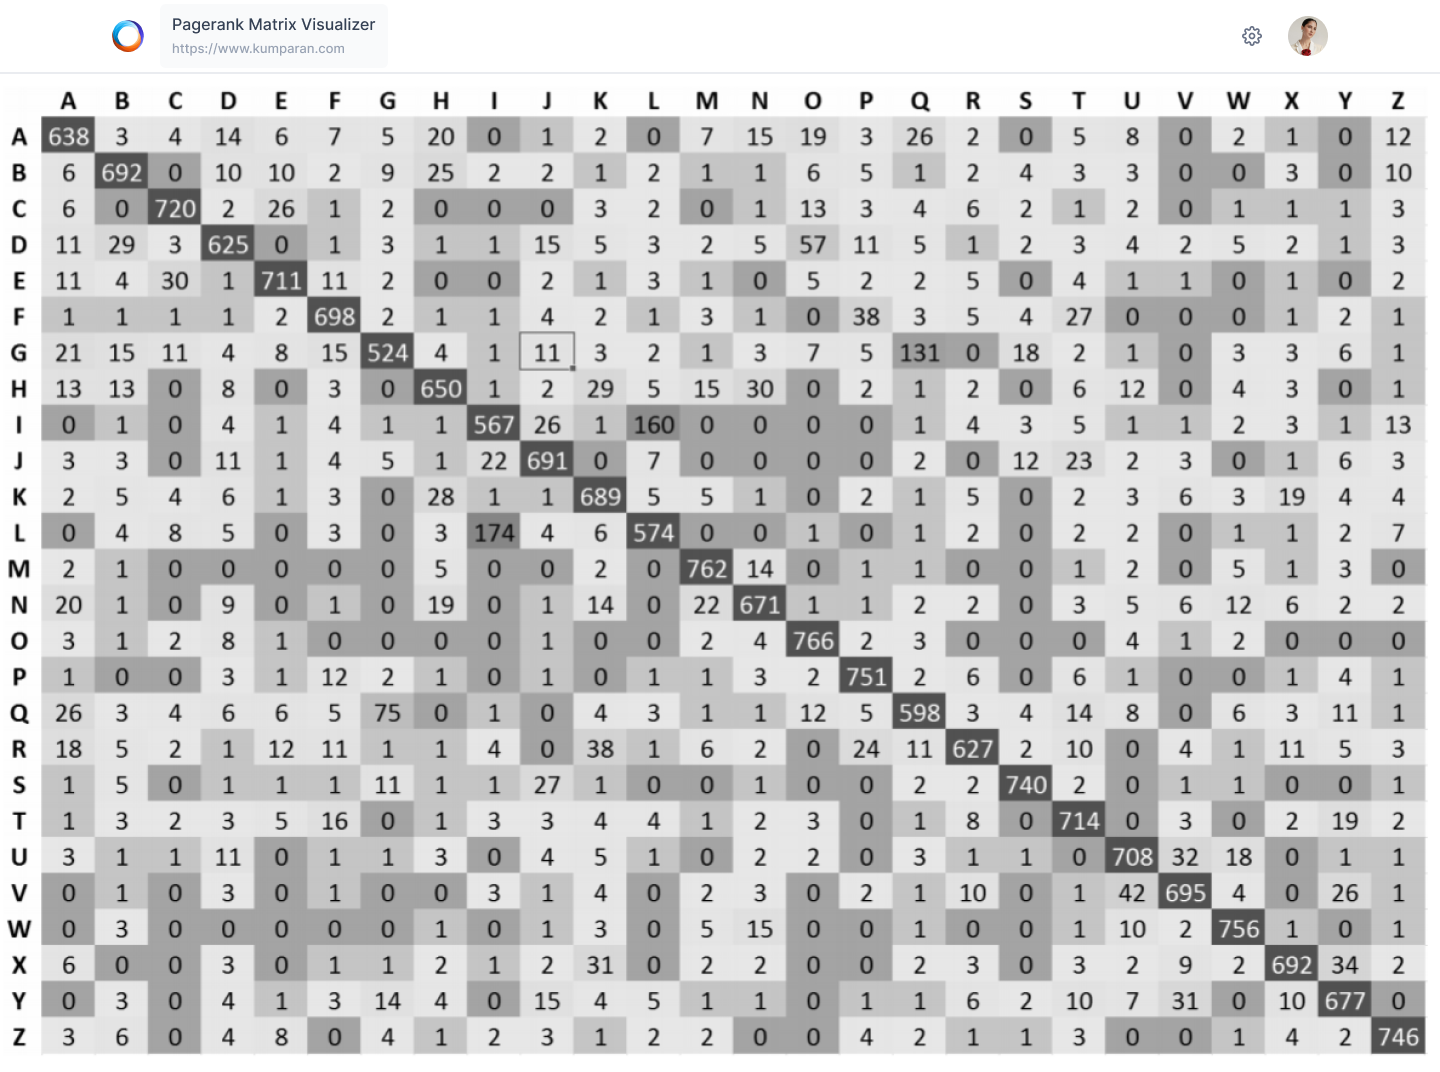
\includegraphics[keepaspectratio, width=13cm]{gambar/page_rank_matrix_visualizer.png}
%	\caption{Desain tampilan \textit{page rank matrix} per-domain atau seluruh domain dalam bentuk dua dimensi}
%	\label{gambar:page_rank_matrix_visualizer.png}
%\end{figure}
%
%\begin{figure}[H]
%	\centering
%	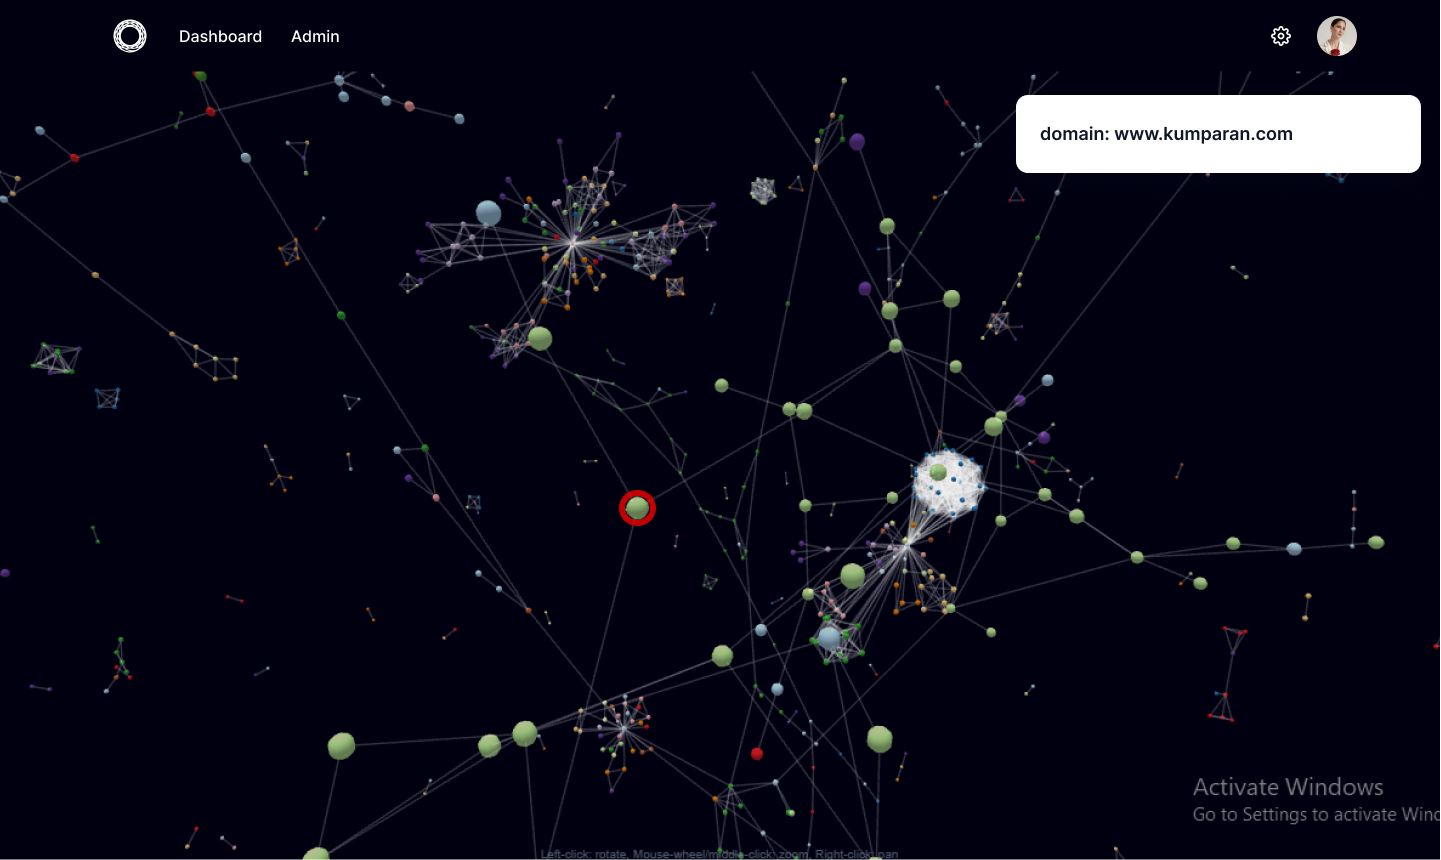
\includegraphics[keepaspectratio, width=13cm]{gambar/pagerank-matrix-3d.png}
%	\caption{Desain tampilan \textit{page rank matrix} per-domain atau seluruh domain dalam bentuk tiga dimensi}
%	\label{gambar:pagerank_matrix_3d.png}
%\end{figure}
%
%
%Adapun routing tabel dari halaman ini adalah sebagai berikut
%
%
%\begin{table}[H]
%	\centering
%	\caption{\textit{Routing Table Halaman Dashboard Admin}}
%	\label{uat}
%	\begin{tabular}{@{} |p{0.5cm}|p{3.5cm}| p{1.5cm}|p{2cm}|p{2cm}|p{2cm} |p{2cm}|p{0.5cm}|@{}}
	%		\hline
	%		\textbf{No.} & \textbf{\textit{Route}} & \textbf{\textit{Method}} & \textbf{\textit{Description}}  & \textbf{\textit{Body}} & \textbf{\textit{Query}} &  \textbf{\textit{Return}} \\
	%		\hline
	%		1 & /pagerank-matrix & GET & Menampilkan halaman matrix dari suatu atau seluruh domain dalam bentuk 2 dimensi atau 3 dimensi & - & type, domain & View \\
	%		\hline
	%	\end{tabular}
%\end{table}
%
%
%\subsection{Halaman Kelola Admin}
%
%Pada halaman kelola admin untuk admin berfokus pada pengelolaan admin pada \textit{search engine} yang telah dibuat. Terdapat beberapa fitur seperti \textit{update} admin, tambah admin, list admin dan pencarian admin. Desain tampilan dibuat seperti daftar berguna untuk memudahkan pengguna dalam menavigasi dari satu admin ke admin yang lainnya.  Halaman ini dibuat tidak memenuhi semua \textit{white spacing} yang tersedia bertujuan agar pengguna lebih mudah dalam menginterpretasikan maksud dan fungsi dari halaman yang sedang dibuka.
%
%\begin{figure}[H]
%	\centering
%	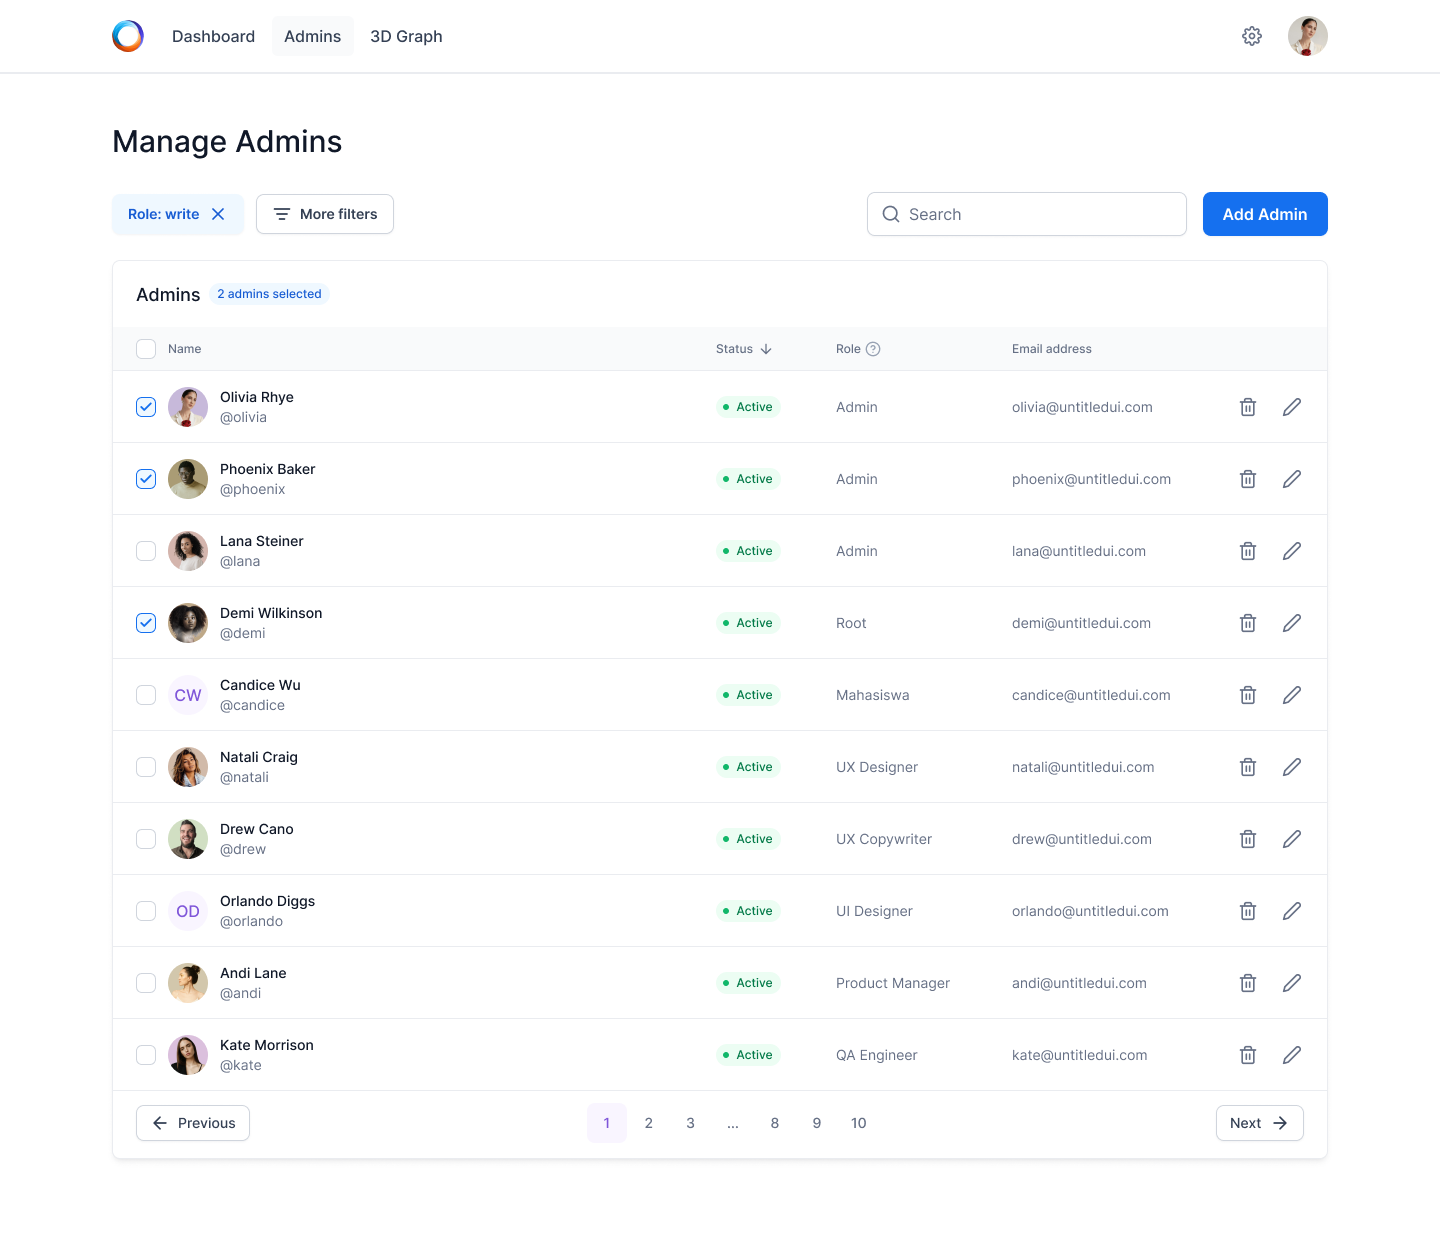
\includegraphics[keepaspectratio, width=13cm]{gambar/managa_admin.png}
%	\caption{Desain tampilan kelola admin \textit{search engine}}
%	\label{gambar:managa_admin.png}
%\end{figure}
%
%Pada tombol tambah admin, admin akan dinavigasikan ke halaman formulir tambah admin.
%
%\begin{figure}[H]
%	\centering
%	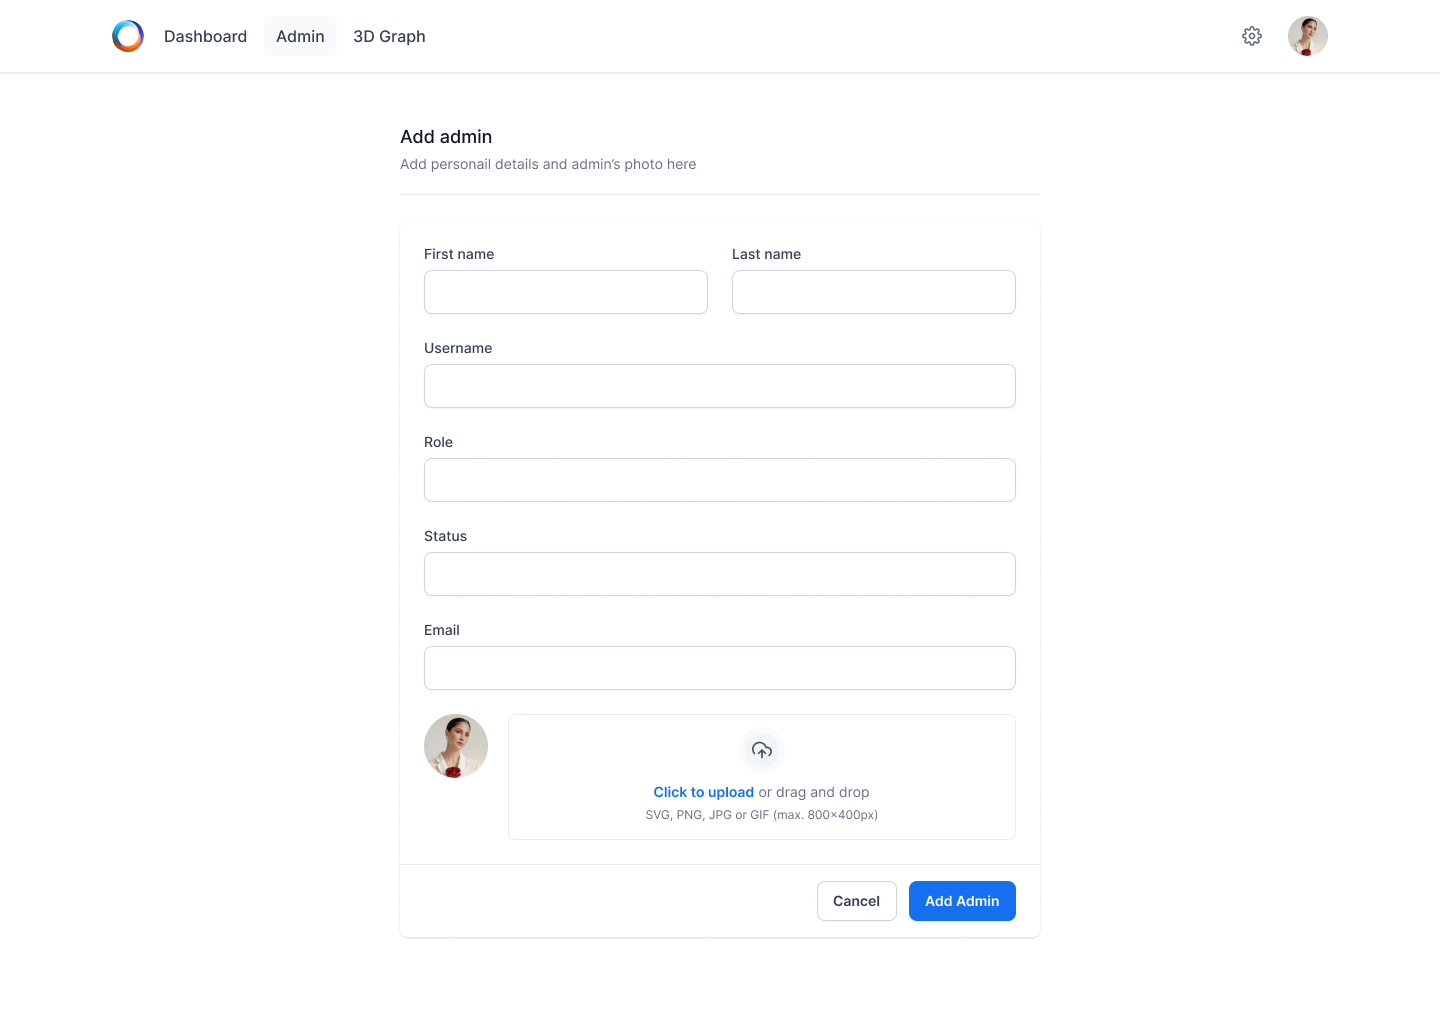
\includegraphics[width=16cm]{gambar/add-admin.png}
%	\caption{Desain tampilan update admin \textit{search engine}}
%	\label{gambar:add-admin.png}
%\end{figure}
%
%Untuk tombol update pada halaman kelola admin, admin akan dinavigasikan ke halaman update admin guna mengupdate informasi mengenai admin.
%
%\begin{figure}[H]
%	\centering
%	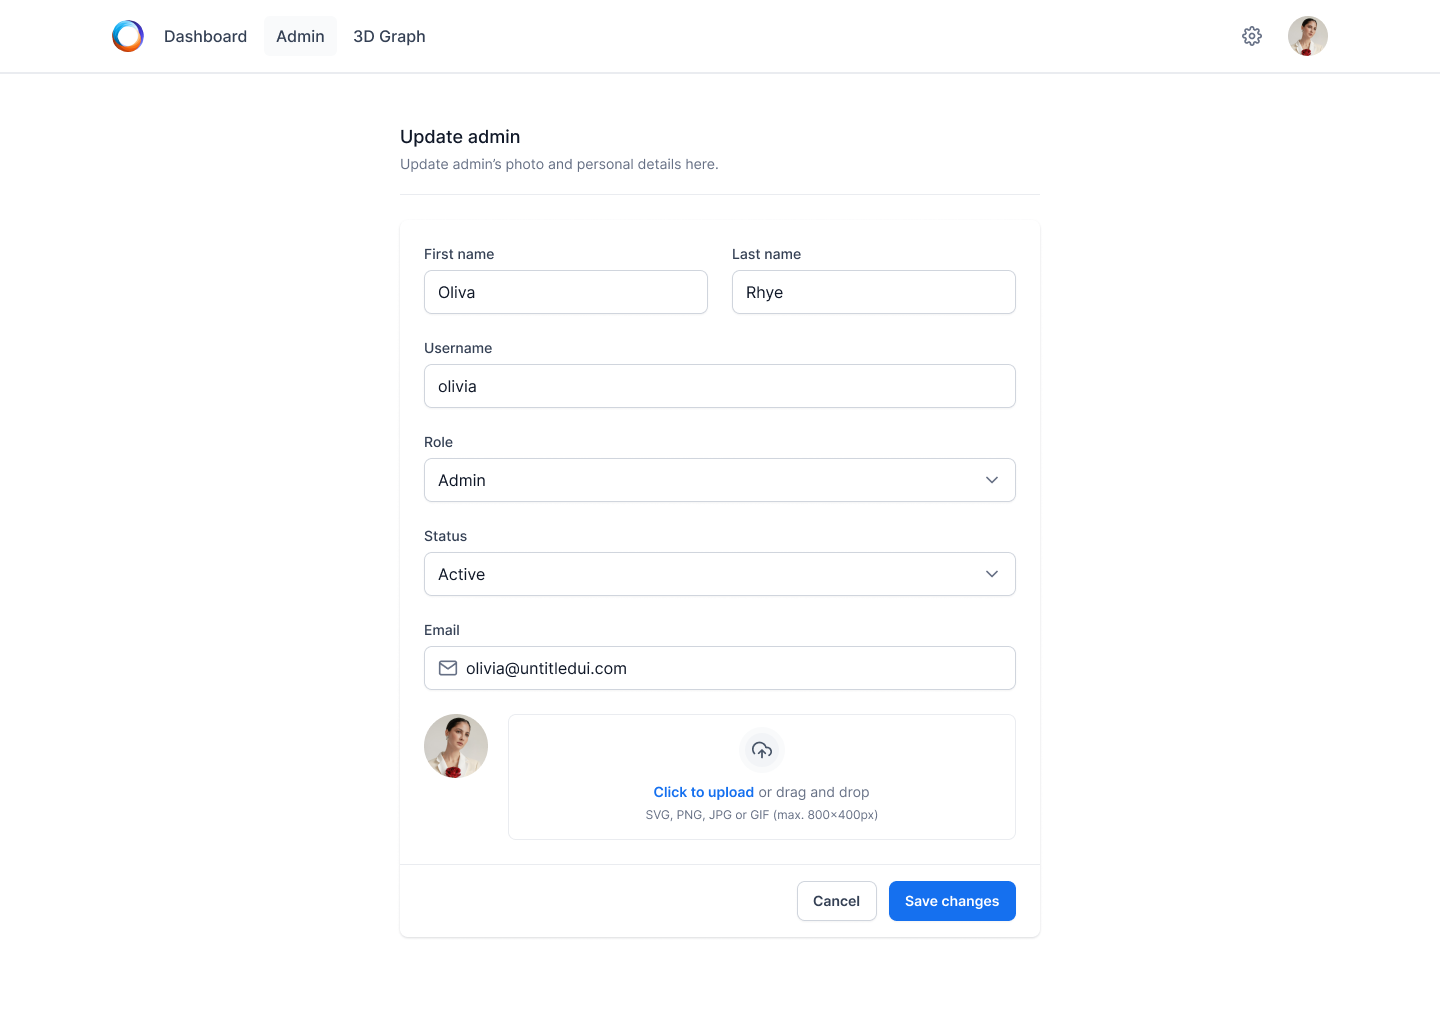
\includegraphics[keepaspectratio, width=13cm]{gambar/login-admin.png}
%	\caption{Desain tampilan update admin \textit{search engine}}
%	\label{gambar:login-admin.png}
%\end{figure}
%
%
%Adapun routing tabel dari halaman ini adalah sebagai berikut
%
%
%\begin{longtable}{@{} |p{0.5cm}|p{3.5cm}| p{1.5cm}|p{2cm}|p{2cm}|p{2cm} |p{2cm}|p{0.5cm}|@{}}
%	\caption{\textit{Routing Table Halaman Dashboard Admin}}\\
%	\hline
%	\textbf{No.} & \textbf{\textit{Route}} & \textbf{\textit{Method}} & \textbf{\textit{Description}}  & \textbf{\textit{Body}} & \textbf{\textit{Query}} &  \textbf{\textit{Return}} \\
%	\hline
%	1 & /api/v1/admins & GET & Mendapatkan daftar admin \textit{crawler} & -  &  page, limit, roles, query& JSON \\
%	\hline
%	2 & /api/v1/admins/:id /delete & DELETE & Menghapus admin & -  &  -&JSON \\
%	\hline
%	3 & /api/v1/admins/:id /update & PATCH & Mengupdate admin & firstName, lastName, username, role, status, email, profilePictureUrl  &  - &JSON \\
%	\hline
%	4 & /api/v1/admins/:id & GET & Mendapatkan data admin & - &  - & JSON \\
%	\hline
%	5 & /api/v1/admins/:id /create & POST & Menambahkan admin & firstName, lastName, username, role, status, email, profilePictureUrl  &  - &JSON \\
%	\hline
%	6 & /dashboard/admins & GET & Menampilkan halaman kelola & - &  - & View \\
%	\hline
%	7 & /dashboard/admins
%	/add & GET & Menampilkan form tambah admin & - &  - & View \\
%	\hline
%	8 & /dashboard/admins
%	/:id/update & GET & Menampilkan form update admin & - &  - & View \\
%	\hline
%\end{longtable}
%
%
%\subsection{Halaman Peta Situs Admin}
%
%Pada halaman peta situs untuk admin, admin dapat melihat semua situs yang berhasil di-\textit{crawling} dalam bentuk graf 3 dimensi. Graf 3 dimensi dipilih agar visualisasi dari semua link terlihat menarik dan mudah untuk dinavigasi oleh pengguna. Titik dari graf ini adalah sebuah situs dan sisi dari grafnya adalah \textit{outgoing link}. Admin juga dapat mengelola \textit{outgoing link} dari sebuah situs dalam halaman ini. Halaman dibuat dalam tema gelap bertujuan untuk menciptakan suasana luar angkasa dengan titik dari graf melambangkan planet planet yang ada di luar angkasa. Halaman ini dapat diakses dengan menekan tombol "\textit{3D Graph}" pada navigasi \textit{header} yang terdapat di atas halaman web.
%
%\begin{figure}[H]
%	\centering
%	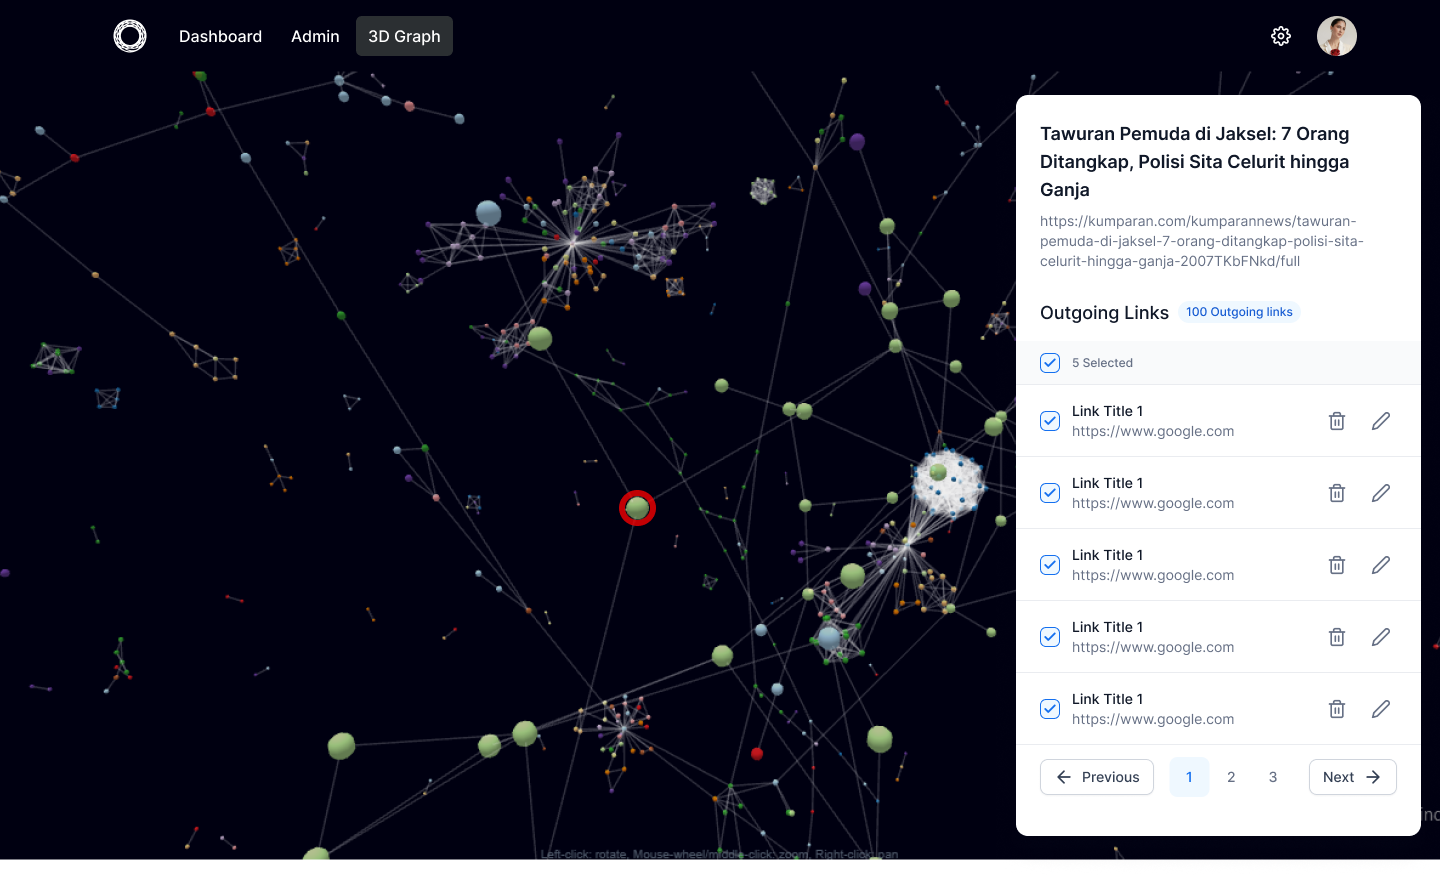
\includegraphics[keepaspectratio, width=13cm]{gambar/admin-sitemap.png}
%	\caption{Desain tampilan peta situs untuk admin \textit{search engine}}
%	\label{gambar:admin-sitemap.png}
%\end{figure}
%
%
%Adapun routing tabel dari halaman ini adalah sebagai berikut
%
%\begin{longtable}{@{} |p{0.5cm}|p{3.5cm}| p{1.5cm}|p{2cm}|p{2cm}|p{2cm} |p{2cm}|p{0.5cm}|@{}}
%	
%	\caption{\textit{Routing Table Halaman Peta Situs Admin}}\\
%	\hline
%	\textbf{No.} & \textbf{\textit{Route}} & \textbf{\textit{Method}} & \textbf{\textit{Description}}  & \textbf{\textit{Body}} & \textbf{\textit{Query}} &  \textbf{\textit{Return}} \\
%	\hline
%	1 & /api/v1/sites/:id
%	/delete & DELETE & Mendelete suatu situs & -  & - & JSON \\
%	\hline
%	2 & /api/v1/sites/:id
%	/update & UPDATE & Mengupdate suatu situs & title, link  & - & JSON \\\hline
%	3 & /api/v1/sites/:id
%	/outgoing & GET & Mendapatkan semua situs outgoing dari suatu situs & -  & limit, page & JSON \\
%	\hline
%	4 & /api/v1/sites/:id & GET & Mendapatkan informasi dari suatu situs & - & - & JSON \\\hline
%	5 & /dashboard/sitemap & GET & Menampilkan halaman peta situs untuk admin & - & site, mode & View \\
%	\hline
%	\hline
%\end{longtable}
%
%
%\subsection{Halaman Login Admin}
%
%Pada halaman login admin, admin dapat login ke dalam \textit{dashboard} admin dengan menggunakan \textit{email} dan password yang telah disediakan. Halaman \textit{login} dibuat menengah agar mata pengguna hanya fokus ke bagian tengah saja dan membuat pengguna lebih mudah menginterpretasikan maksud dan fungsi dari halaman yang sedang dibuka.
%
%\begin{figure}[H]
%	\centering
%	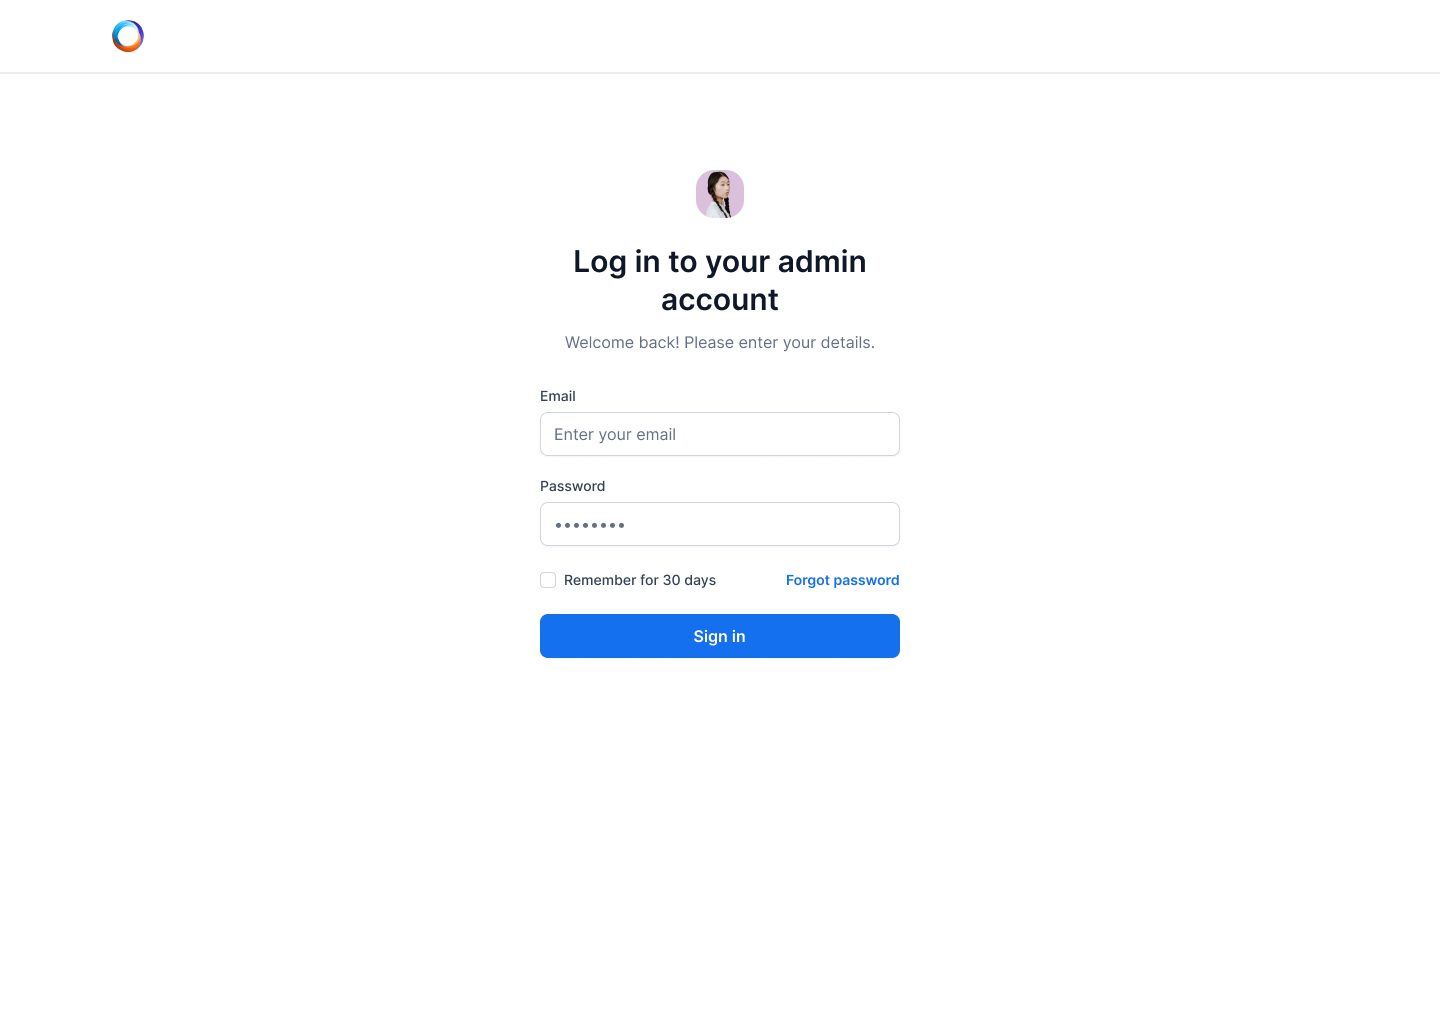
\includegraphics[keepaspectratio, width=13cm]{gambar/admin-login-page.png}
%	\caption{Desain tampilan \textit{login} admin \textit{search engine}}
%	\label{gambar:admin-login-page.png}
%\end{figure}
%
%
%\begin{table}[H]
%	\centering
%	\caption{\textit{Routing Table Halaman Dashboard Admin}}
%	\label{uat}
%	\begin{tabular}{@{} |p{0.5cm}|p{3.5cm}| p{1.5cm}|p{2cm}|p{2cm}|p{2cm} |p{2cm}|p{0.5cm}|@{}}
	%		\hline
	%		\textbf{No.} & \textbf{\textit{Route}} & \textbf{\textit{Method}} & \textbf{\textit{Description}}  & \textbf{\textit{Body}} & \textbf{\textit{Query}} &  \textbf{\textit{Return}} \\
	%		\hline
	%		1 & /api/v1/login & GET & Mendapatkan daftar admin \textit{crawler} & email, password  & - & JSON \\ \hline
	%		2 & /dashboard/login & POST & Menampilkan halaman login dashboard untuk admin & - & - & View \\
	%		\hline
	%	\end{tabular}
%\end{table}
%
%\subsection{Halaman Pencarian Pengguna}
%
%Pada halaman pencarian untuk pengguna, pengguna dapat melakukan pencarian pada halaman ini. Terdapat dua menu pada bagian \textit{header} yang dapat pengguna akses yaitu ranking situs dan peta web. Pada halaman ini juga disediakan pencarian pengguna sebelumnya. Bagian \textit{recent searches} betujuan untuk memudahkan pengguna dalam mencari kata pencarian yang pernah dicari sebelumnya. Halaman ini dibuat tidak memenuhi \textit{white spacing} yang tersedia bertujuan agar pengguna lebih mudah dalam menginterpretasikan maksud dan fungsi dari halaman yang sedang dibuka.  Halaman ini dibuat tidak memenuhi semua \textit{white spacing} yang tersedia bertujuan agar pengguna lebih mudah dalam menginterpretasikan maksud dan fungsi dari halaman yang sedang dibuka.
%
%\begin{figure}[H]
%	\centering
%	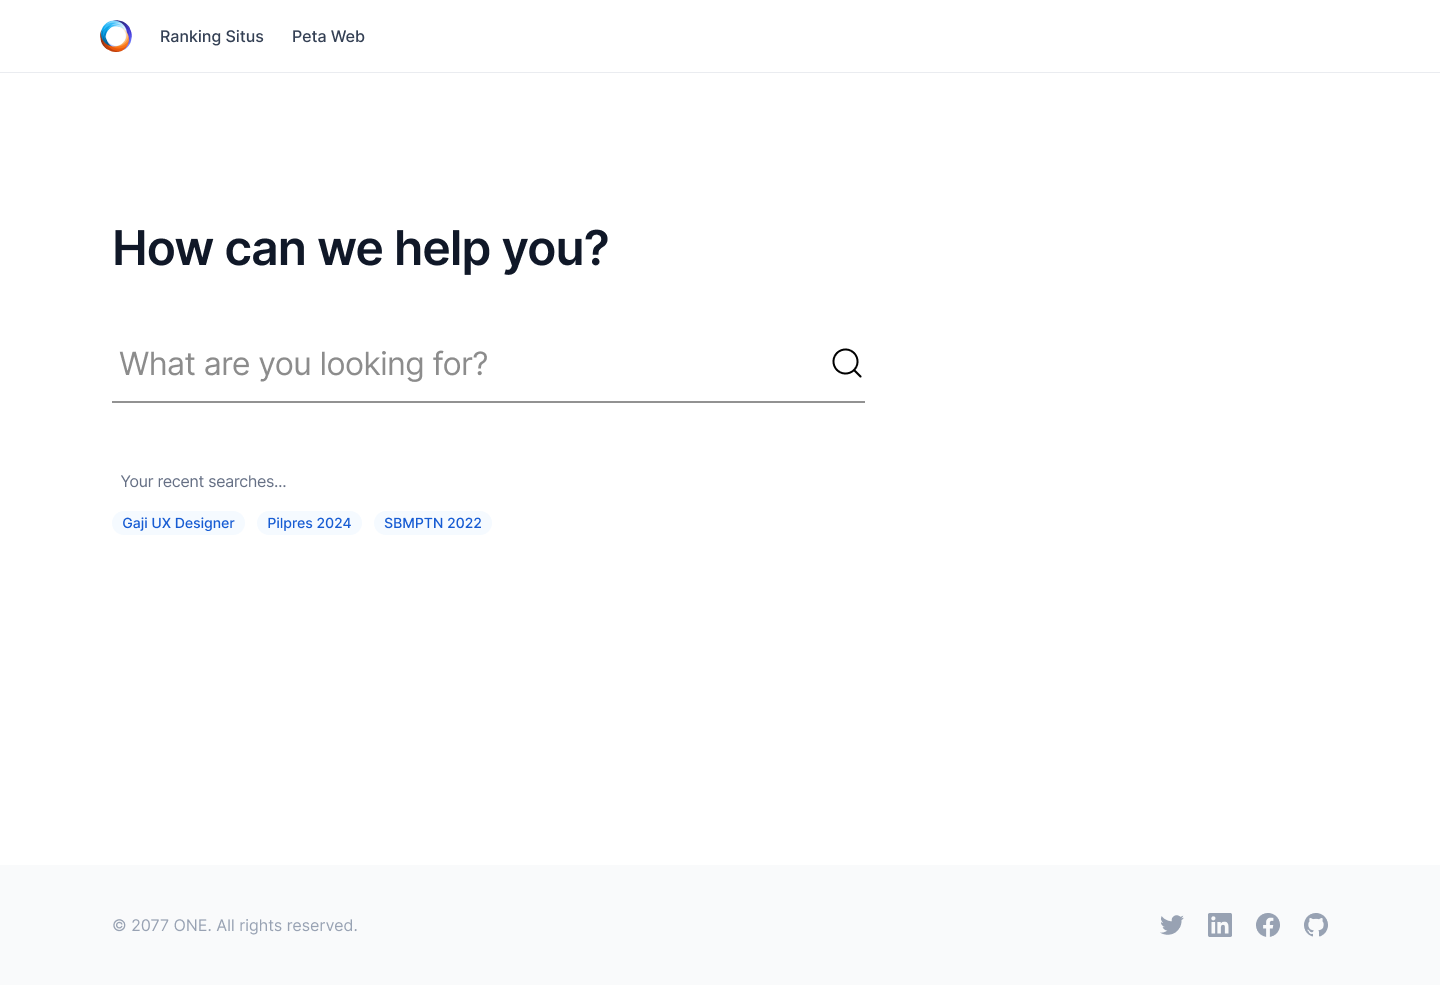
\includegraphics[keepaspectratio, width=13cm]{gambar/user-search-page.png}
%	\caption{Desain tampilan halaman pencarian untuk pengguna}
%	\label{gambar:user-search-page.png}
%\end{figure}
%
%
%\begin{table}[H]
%	\centering
%	\caption{\textit{Routing Table Halaman Pencarian Pengguna}}
%	\label{uat}
%	\begin{tabular}{@{} |p{0.5cm}|p{3.5cm}| p{1.5cm}|p{2cm}|p{2cm}|p{2cm} |p{2cm}|p{0.5cm}|@{}}
	%		\hline
	%		\textbf{No.} & \textbf{\textit{Route}} & \textbf{\textit{Method}} & \textbf{\textit{Description}}  & \textbf{\textit{Body}} & \textbf{\textit{Query}} &  \textbf{\textit{Return}} \\
	%		\hline
	%		1 & /api/v1/search & GET & Mendapatkan daftar admin \textit{crawler} & - & - & query \\ \hline
	%		2 & / & GET & Menapilkan halaman pencarian untuk pengguna & - & - & View \\
	%		\hline
	%	\end{tabular}
%\end{table}
%
%\subsection{Halaman Peta Situs Pengguna}
%
%Sama seperti peta situs untuk admin, pengguna dapat melihat semua situs yang berhasil di-\textit{crawling} dalam bentuk graf 3 dimensi. Graf 3 dimensi dipilih agar visualisasi dari semua link terlihat menarik dan mudah untuk dinavigasi oleh pengguna. Titik dari graf ini adalah sebuah situs dan sisi dari grafnya adalah \textit{outgoing link}. Pengguna dapat melihat \textit{outgoing link} dari sebuah situs yang difokuskan pada bagian kanan layar. Pengguna juga dapat memfokuskan \textit{link} yang lain dengan menekan salah satu dari titik titik yang ada. Halaman dibuat dalam tema gelap bertujuan untuk menciptakan suasana luar angkasa dengan titik dari graf melambangkan planet planet yang ada di luar angkasa.
%
%\begin{figure}[H]
%	\centering
%	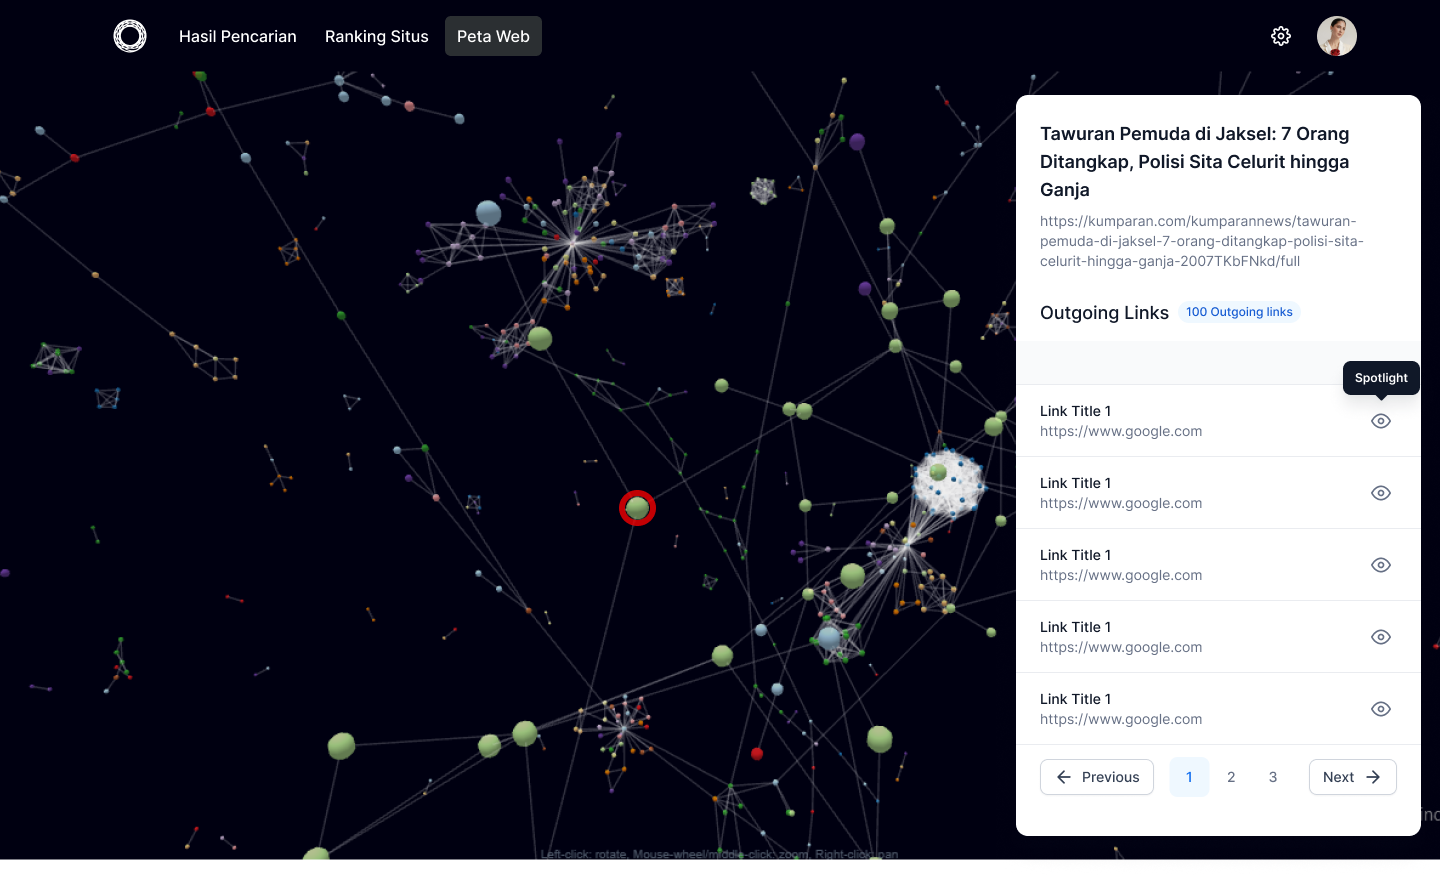
\includegraphics[keepaspectratio, width=13cm]{gambar/user-sitemap.png}
%	\caption{Desain tampilan peta situs untuk pengguna \textit{search engine}}
%	\label{gambar:user-sitemap.png}
%\end{figure}
%
%
%Adapun routing tabel dari halaman ini adalah sebagai berikut
%
%\begin{table}[H]
%	\centering
%	\caption{\textit{Routing Table Halaman Peta Situs Pengguna}}
%	\label{uat}
%	\begin{tabular}{@{} |p{0.5cm}|p{3.5cm}| p{1.5cm}|p{2cm}|p{2cm}|p{2cm} |p{2cm}|p{0.5cm}|@{}}
	%		\hline
	%		\textbf{No.} & \textbf{\textit{Route}} & \textbf{\textit{Method}} & \textbf{\textit{Description}}  & \textbf{\textit{Body}} & \textbf{\textit{Query}} &  \textbf{\textit{Return}} \\
	%		\hline
	%		1 & /api/v1/sites/:id
	%		/outgoing & GET & Mendapatkan semua situs outgoing dari suatu situs & -  & limit, page & JSON \\
	%		\hline
	%		2 & /api/v1/sites/:id & GET & Mendapatkan informasi dari suatu situs & - & - & JSON \\\hline
	%		3 & /sitemap & GET & Menampilkan halaman peta situs untuk pengguna  & - & site, mode & View \\
	%		\hline
	%	\end{tabular}
%\end{table}
%
%\subsection{Halaman Hasil Pencarian Pengguna}
%
%Halaman ini merupakan halaman setelah pengguna mamasukan kata pencarian pada \textit{search engine}. Pada halaman ini menyajikan situs-situs yang relevan berdasarkan kata pencarian yang pengguna berikan. Pengguna juga dapat menambahkan parameter tambahan seperti \textit{sort by} dan sebuah \textit{filter} untuk membuat hasil pencarian lebih akurat untuk pengguna. Hasil pencarian dibuat tidak mengisi seluruh \textit{white space} agar pengguna lebih mudah menavigasi hasil pencarian dengan mengurangi pergerakan mata pengguna. Pada hasil pencarian juga disediakan tombol tanda panah miring bertujuan untuk mengantarkan pengguna ke halaman peta situs dan melihat situs hasil pencarian tersebut dalam  bentuk tiga dimensi. Halaman ini dibuat tidak memenuhi semua \textit{white spacing} yang tersedia bertujuan agar pengguna lebih mudah dalam menginterpretasikan maksud dan fungsi dari halaman yang sedang dibuka.
%
%\begin{figure}[H]
%	\centering
%	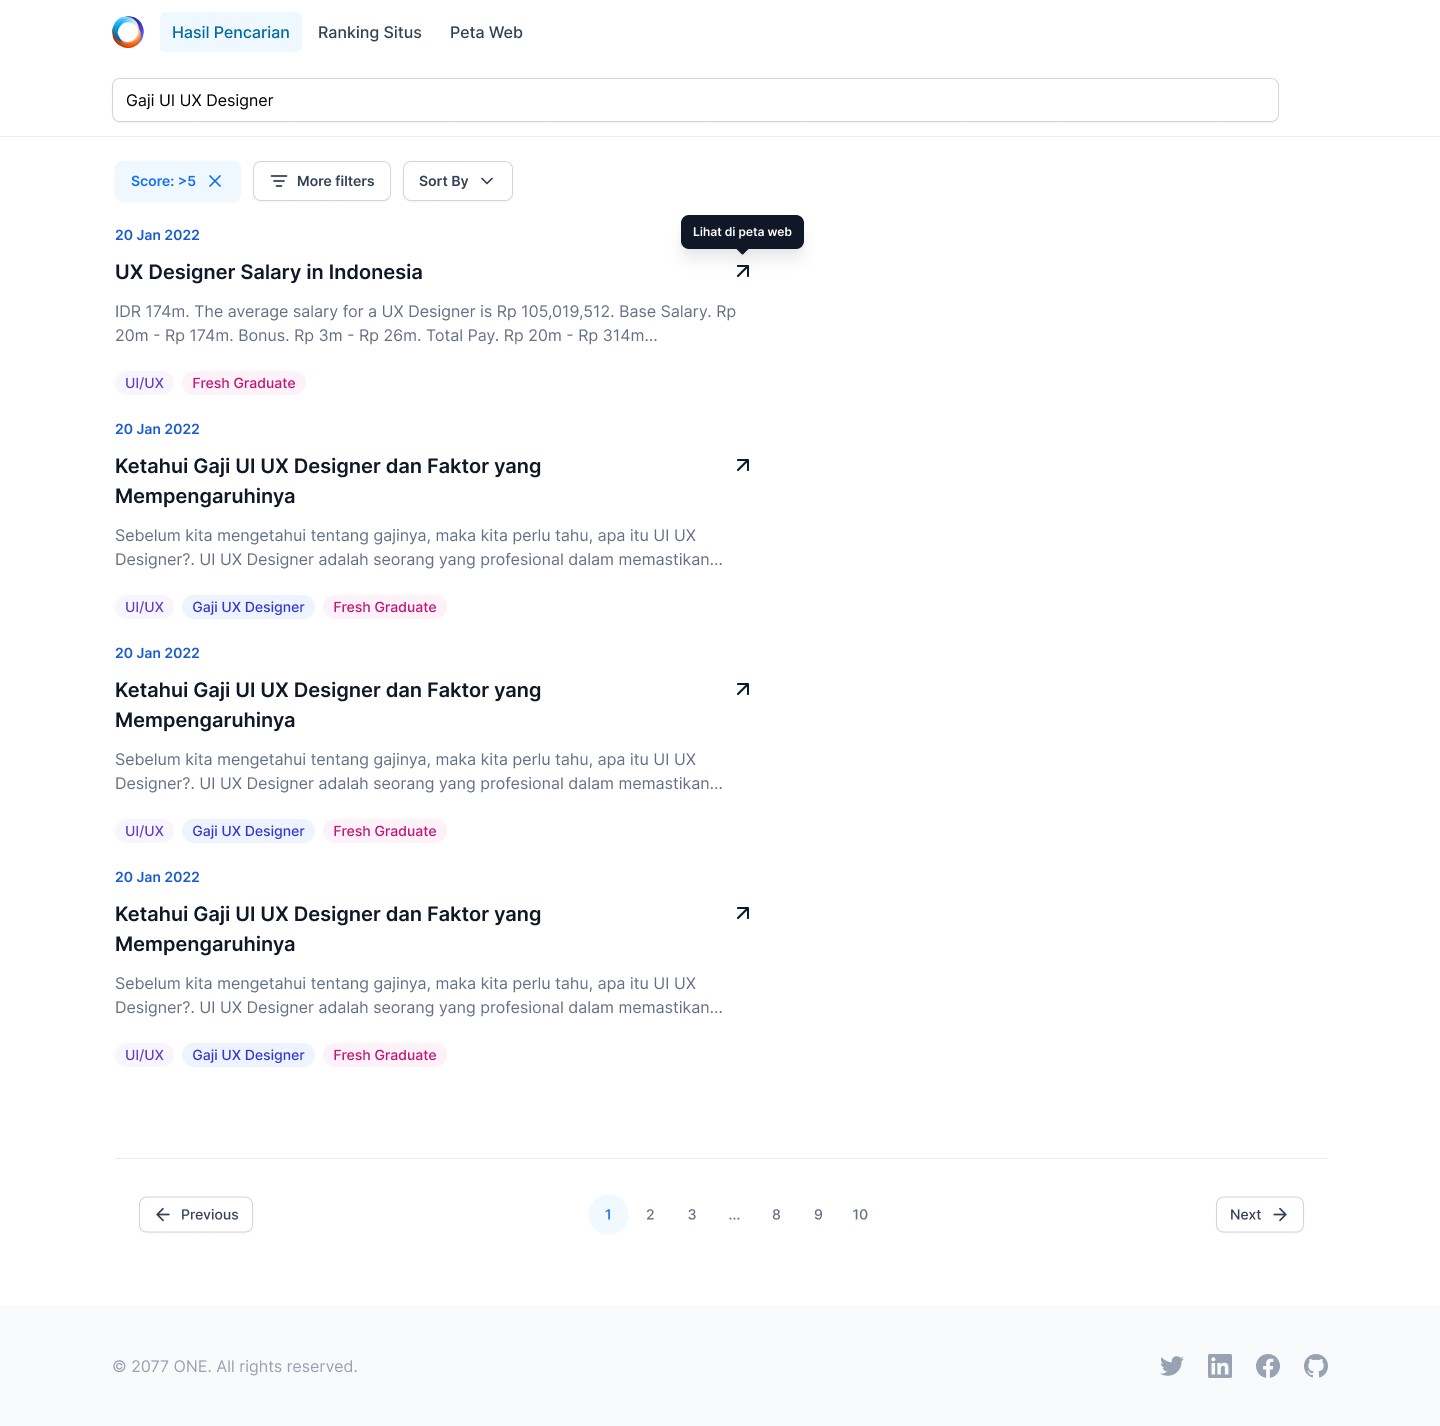
\includegraphics[keepaspectratio, width=10cm]{gambar/user-search-result.png}
%	\caption{esain tampilan halaman hasil pencarian}
%	\label{gambar:user-search-result.png}
%\end{figure}
%
%
%Adapun routing tabel dari halaman ini adalah sebagai berikut
%
%\begin{longtable}{@{} |p{0.5cm}|p{3.5cm}| p{1.5cm}|p{2cm}|p{2cm}|p{2cm} |p{2cm}|p{0.5cm}|@{}}
%	
%	\caption{\textit{Routing Table Halaman Hasil Pencarian Pengguna}}\\
%	\hline
%	\textbf{No.} & \textbf{\textit{Route}} & \textbf{\textit{Method}} & \textbf{\textit{Description}}  & \textbf{\textit{Body}} & \textbf{\textit{Query}} &  \textbf{\textit{Return}} \\
%	\hline
%	1 & /api/v1/search
%	/outgoing & GET & Mendapatkan semua situs yang terkait dengan kata kunci yang diberikan & -  & limit, page, query, filters, sort & JSON \\
%	\hline
%	2 & /search & GET & Menampilkan halaman hasil pencarian berdasarkan kata kunci yang diberikan & - & limit, page, query, filters, sort & View \\\hline
%\end{longtable}
%
%
%\subsection{Halaman Ranking Situs}
%
%Pada halaman ini akan menampilkan ranking dari semua url yang berhasil di-\textit{crawl}. Halaman perankingan situs dibuat tidak mengisi seluruh \textit{white space} agar pengguna lebih mudah menavigasi ranking situs dengan mengurangi pergerakan mata pengguna. Pada ranking juga disediakan tombol tanda panah miring bertujuan untuk mengantarkan pengguna ke halaman peta situs dan melihat situs hasil pencarian tersebut dalam  bentuk tiga dimensi. Halaman ini dibuat tidak memenuhi \textit{white spacing} yang tersedia bertujuan agar pengguna lebih mudah dalam menginterpretasikan maksud dan fungsi dari halaman yang sedang dibuka.
%
%\begin{figure}[H]
%	\centering
%	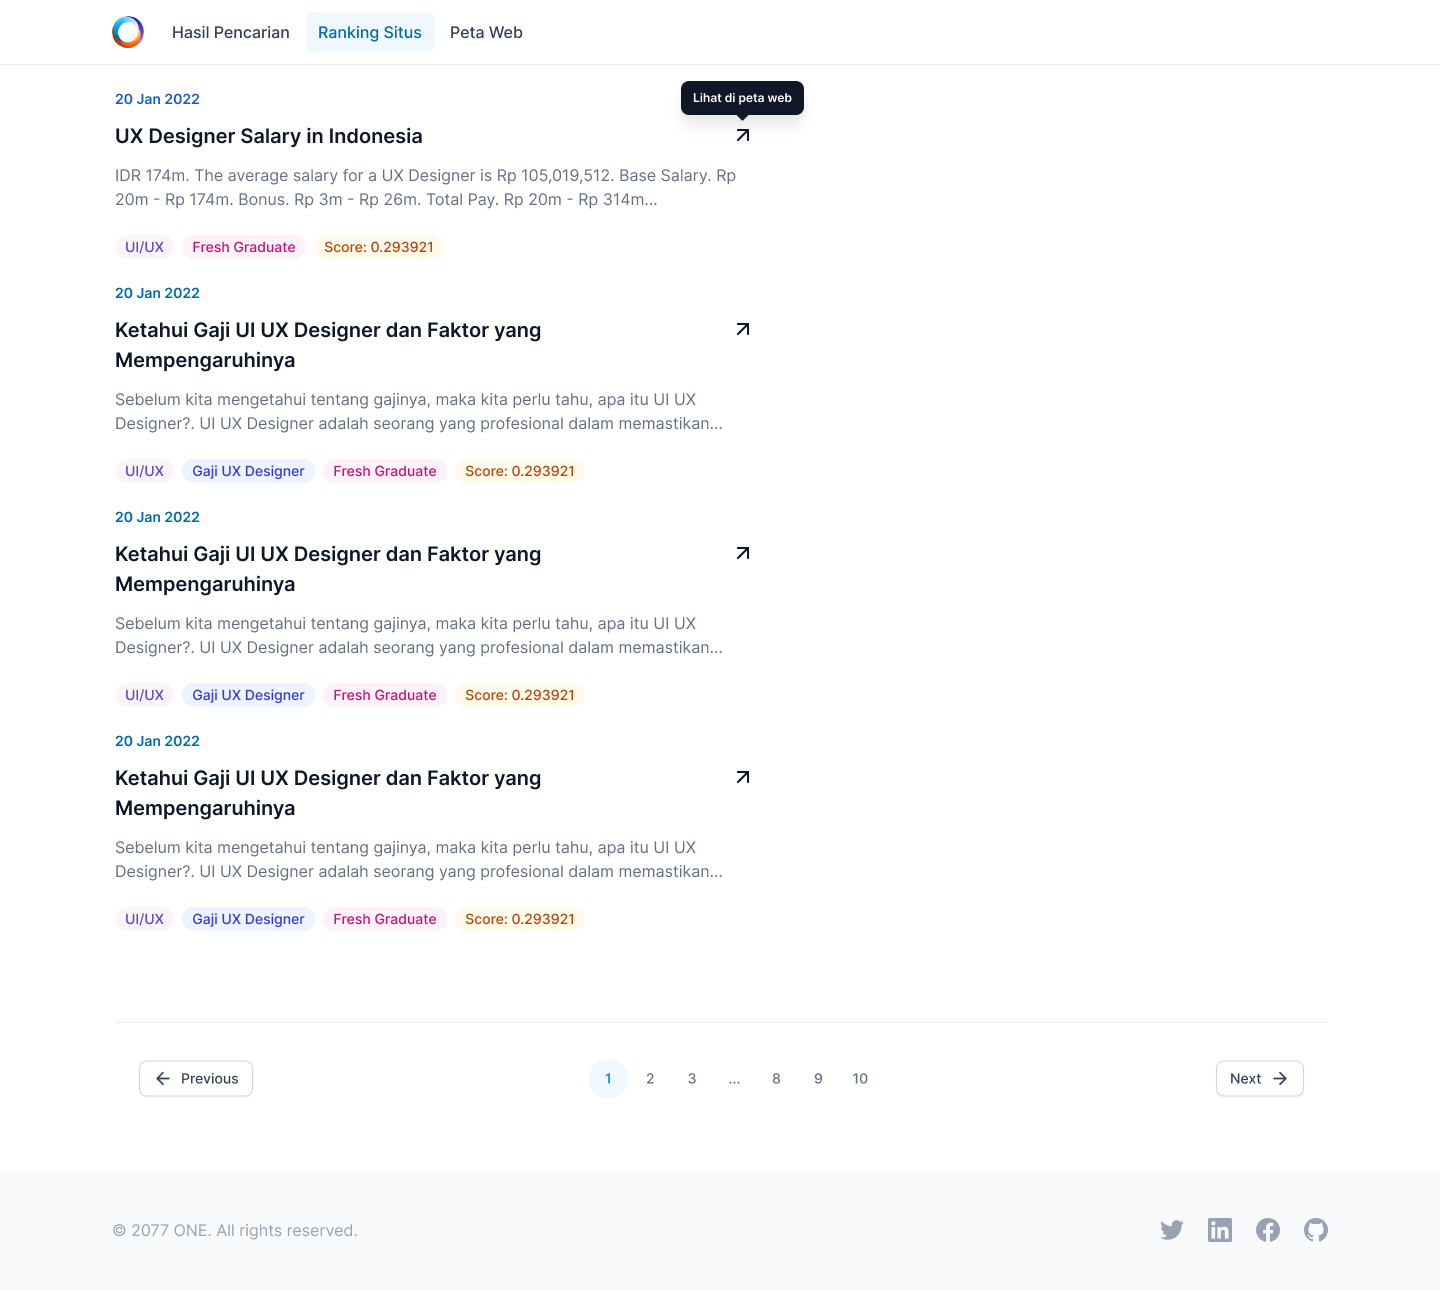
\includegraphics[keepaspectratio, width=13cm]{gambar/user-page-ranking-page.png}
%	\caption{Desain tampilan ranking halaman}
%	\label{gambar:user-page-ranking-page.png}
%\end{figure}
%
%
%
%Adapun routing tabel dari halaman ini adalah sebagai berikut
%
%\begin{table}[H]
%	\centering
%	\caption{\textit{Routing Table Halaman Peta Situs Pengguna}}
%	\label{uat}
%	\begin{tabular}{@{} |p{0.5cm}|p{3.5cm}| p{1.5cm}|p{2cm}|p{2cm}|p{2cm} |p{2cm}|p{0.5cm}|@{}}
	%		\hline
	%		\textbf{No.} & \textbf{\textit{Route}} & \textbf{\textit{Method}} & \textbf{\textit{Description}}  & \textbf{\textit{Body}} & \textbf{\textit{Query}} &  \textbf{\textit{Return}} \\
	%		\hline
	%		1 & /api/v1/ranking
	%		/outgoing & GET & Mendapatkan ranking dari semua situs  & -  & limit, page & JSON \\
	%		\hline
	%		2 & /ranking  & GET & Menampilkan halaman ranking situs & - & limit, page, query, filters, sort & View \\\hline
	%	\end{tabular}
%\end{table}


%
%Pada penelitian ini akan digunakan algoritma \textit{page ranking} DPC yang telah dikembangkan oleh \citep{farhan} menggantikan algoritma \textit{PageRank} yang digunakan oleh \citep{lazu}. Penggantian algoritma untuk \textit{PageRank} ini dimulai dengan mengumpulkan informasi berupa fungsi yang bertanggung jawab atas kewajiban \textit{page rank} dan memodifikasi fungsi-fungsi tersebut untuk mendukung algoritma \textit{page ranking} DPC yang sebelumnya telah dibuat oleh \citep{farhan}.
%
%Sebelumnya, telah dibahas mengenai perbandingan performa dari penggunaan MySQL dengan MongoDB dalam hal pemrosesan \textit{query} dalam jumlah besar yang menyimpulkan bahwa MongoDB lebiih performan dibandingkan MySQL dalam hal pemrosesan query dalam jumlah besar. Pada penelitian ini akan dilakukan proses migrasi dari database sebelumnya yang digunakan penelitian sebelumnya yaitu MySQL ke MongoDB. Pada proses ini akan dikembangkan suatu \textit{script} untuk melakukan migrasi data dari MySQL ke MongoDB dan akan dilakukan modifikasi dan penambahan kode kepada kode penelitian \citep{lazu} agar mendukung penyimpanan ke dalam database MongoDB. Pengkonversian database dari MySQL ke MongoDB meliputi seluruh tabel yang ada dalam database MySQL sebelumnya dengan tambahan beberapa tabel untuk mendukung fitur kelola oleh admin diantaranya sebagai berikut.
%
%
%\begin{table}[H]
%	\centering
%	\caption{Skema Tabel Admin}
%	\label{uat}
%	\begin{tabular}{@{} |p{3cm}|p{3cm}|@{}}
	%		\hline
	%		\textbf{Nama Kolom} & \textbf{Tipe data} \\
	%		\hline
	%		email & \textit{string} \\
	%		\hline
	%		id & \textit{string} (PK) \\
	%		\hline
	%		password & \textit{string} \\
	%		\hline
	%		role & \textit{string} \\
	%		\hline
	%	\end{tabular}
%\end{table}

\section {Analisis Kebutuhan}

Analisis kebutuhan dilakukan guna mengumpulkan informasi mengenai kebutuhan fitur aplikasi dan prioritas fitur aplikasi yang akan dibuat. Dari analisis kebutuhan yang dilakukan dihasilkan sebuah \textit{usecase diagram} yang didefinisikan sebagai berikut.

\begin{figure}[H]
	\centering
	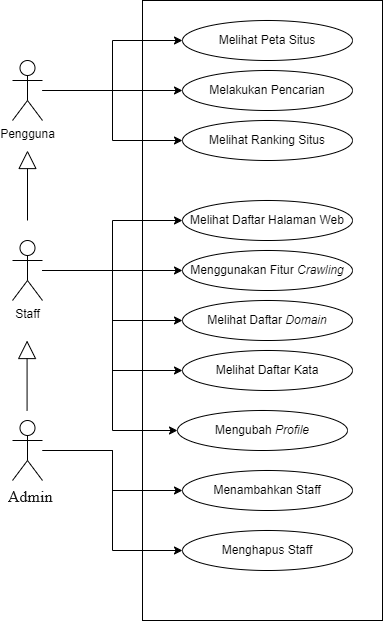
\includegraphics[keepaspectratio, width=8cm]{gambar/usecase.png}
	\caption{\textit{Use Case Diagram}}
	\label{gambar:usecase.png}
\end{figure}


\section {Pengujian Sistem}

Pengujian pada \textit{search engine} menggunakan dua macam pengujian yaitu \textit{User Acceptance Test} atau UAT dan \textit{Unit Testing}. UAT akan dilaksanakan oleh pengguna dengan \textit{scrum master} untuk mengetahui apakah aplikasi sudah sesuai kebutuhan dan layak digunakan. Pengujian \textit{Unit Testing} akan dilakukan oleh tim internal \textit{developer} untuk memastikan fitur-fitur yang telah dikembangkan berjalan dengan baik.
\begin{enumerate}[leftmargin=1\parindent]
	\item \textit{\textbf{Unit Testing}}
	
	\textit{Unit Testing} yang akan dibuat akan mengacu berdasarkan \textit{product backlog} yang telah dibuat sebelumnya. Adapun skenario dari \textit{unit testing} yang akan dilaksanakan pada penelitian ini sebagai berikut.
	
	\begin{longtable}{@{}|p{4cm}|p{8cm}|@{}}
		\caption{\textit{Unit Testing} Tampilan Crawling}\\
		\hline
		\multicolumn{2}{|c|}{\textbf{Unit Testing}} \\
		\hline
		\textbf{Uji Fitur} & \textbf{Skenario Pengujian} \\
		\hline
		Pencarian Pengguna & Pada tampilan halaman pencarian, ketika pengguna memasukkan kata kunci pencarian dan menekan tombol \textit{enter} maka pengguna akan dialihkan ke halaman hasil pencarian \\
		\hline
		Hasil Pencarian & Saat menekan \textit{tab} peta situs atau \textit{sitemap} maka akan ditampilkan peta situs dari kata kunci yang sedang dicari \\
		\cline{2-2} 
		& Pengguna dapat memasukkan kata kunci pencarian dengan memasukkan \textit{query} dengan kunci \textit{search} untuk mendapatkan hasil pencarian \\
		\hline
		Peta Situs & Pengguna dapat memasukkan kata kunci ulang dengan memasukkan kata kunci pada \textit{text field} di pojok kanan atas lalu menekan tombol \textit{enter} \\
		\cline{2-2}
		& Pengguna dapat mem-\textit{filter} peta situs berdasarkan negara dengan memilih negara pada tombol \textit{Select Countries} di pojok kanan atas \\
		\cline{2-2}
		& Pengguna dapat memasukkan kata kunci pencarian dengan memasukkan kata kunci pencarian pada \textit{query} URL dengan kunci \textit{query} dan negara dengan kunci \textit{countries} \\
		\hline
		Login & Ketika pengguna memasukkan informasi akun dengan benar ke dalam formulir yang ada maka pengguna akan dialihkan ke halaman \textit{dashboard} \\
		\cline{2-2}
		& Ketika pengguna memasukkan informasi akun dengan salah ke dalam formulir yang ada maka pengguna akan diberi pesan bahwa pengguna memasukkan informasi akun yang salah \\	
		\hline
		Dashboard & Ketika pengguna menekan tombol \textit{profile} maka pengguna akan disajikan \textit{popup} yang berisi aksi \textit{logout}\\
		\hline
		Page Ranking & Ketika pengguna menekan tombol \textit{start}, maka \textit{status page ranking} akan berubah menjadi \textit{running} dan akan muncul tombol \textit{stop} \\
		\cline{2-2}	
		& Ketika pengguna menekan tombol \textit{stop}, maka \textit{page ranking} akan berhenti dan tombol \textit{start} akan muncul \\
		\hline
		Crawling & Ketika pengguna menekan tombol \textit{start}, maka \textit{status crawling} akan berubah menjadi \textit{running} dan akan muncul tombol \textit{stop} \\
		\cline{2-2}
		& Ketika pengguna menekan tombol \textit{stop}, maka \textit{crawling} akan berhenti dan tombol \textit{start} akan muncul \\
		\cline{2-2}
		& Saat \textit{tab} \textit{domains} diklik, pengguna akan dialihkan ke sub halaman daftar domain \\
		\cline{2-2}
		& Saat \textit{tab} \textit{webpages} diklik, pengguna akan dialihkan ke sub halaman daftar \textit{webpages} \\
		\hline
		Daftar Situs & Ketika pengguna menekan salah satu situs pada daftar situs, pengguna akan dialihkan ke halaman detail situs \\
		\cline{2-2}
		& Pengguna dapat menyaring daftar \textit{situs} yang dimunculkan dengan mengaplikasikan \textit{filter} yang tersedia yang terletak di atas tabel \\
		\hline
		Daftar \textit{Domain} & Pengguna dapat menyaring daftar \textit{domain} yang dimunculkan dengan mengaplikasikan \textit{filter} yang tersedia yang terletak di atas tabel \\
		\hline
		\textit{Document Ranking} & Ketika pengguna menekan tombol \textit{start}, maka \textit{status document ranking} akan berubah menjadi \textit{running} dan akan muncul tombol \textit{stop} \\
		\cline{2-2}
		& Ketika pengguna menekan tombol \textit{stop}, maka \textit{document ranking} akan berhenti dan tombol \textit{start} akan muncul \\
		\cline{2-2}
		\hline
		\hline
		& Ketika pengguna menekan \textit{tab} \textit{words}, maka akan dialihkan ke sub halaman \textit{words} \\
		\cline{2-2}		

		& Ketika pengguna menekan \textit{tab} \textit{search log}, maka akan dialihkan ke sub halaman \textit{search log} \\
		\hline
		Daftar Staff & Ketika tombol \textit{create new staff} ditekan, maka akan dialihkan ke halaman tambah \textit{staff} baru \\
		\cline{2-2}
		&  Ketila tombol \textit{more} yang dilambangkan dengan ikon tiga titik vertikal ditekan, maka akan muncul \textit{popup} yang berisi aksi \textit{delete staff}. \\
		\cline{2-2}
		& Ketika \textit{delete staff} ditekan, maka \textit{staff} akan dihapus dari daftar \textit{staff} setelah melakukan \textit{refresh} ulang. \\
		\hline
		Tambah Staff & Ketika form berhasil diisi maka \textit{staff} baru akan ditambahkan ke daftar \textit{staff} \\
		\hline
	\end{longtable}

	\item \textit{\textbf{User Acceptance Test}}
	
	\textit{User Acceptance Testing} dibuat berdasarkan fitur-fitur yang dapat diakses oleh pengguna pada \textit{product backlog} yang telah dibuat sebelumnya. Untuk format \textit{User Acceptance Test} digunakan format sebagai berikut. Kolom kesesuaian dibagi menjadi dua yaitu Setuju dan Tidak Setuju
	
	\begin{longtable}{@{}|p{0.5cm}|p{5cm}|p{3cm}|p{3cm}|p{2cm}|@{}}
		
		\caption{Format Pengujian \textit{User Acceptance Test}}\\
		\hline
		\multirow{2}{5cm}{\textbf{No}} & \multirow{2}{5cm}{\textbf{\textit{Acceptance Requirements}}} & \multicolumn{2}{c|}{\textbf{Kesesuaian}} &	 \\
		\cline{3-4}
		\textbf{} & \textbf{\textit{}} & \textbf{Setuju} & \textbf{Tidak Setuju} & \textbf{Keterangan} \\
		\hline
		1 & Fitur pencarian pengguna sudah sesuai dengan kebutuhan pengguna &  & & \\
		\hline
		2 & Fitur hasil pencarian sudah sesuai dengan kebutuhan &  & & \\
		\hline
		3 & Fitur \textit{login} sudah sesuai kebutuhan &  & &   \\
		\hline
		4 & Fitur \textit{dashboard} sudah sesuai kebutuhan &  & & \\
		\hline
		5 & Fitur \textit{peta situs} sudah sesuai kebutuhan  &  &  & \\
		\hline
		6 & Fitur \textit{crawling} sudah sesuai kebutuhan &  &  & \\
		\hline
		7 & Fitur \textit{page ranking} sudah sesuai kebutuhan & &  & \\
		\hline
		
		8 & Fitur \textit{document ranking} sudah sesuai kebutuhan & &  &  \\
		\hline
		9 & Fitur \textit{daftar situs} sudah sesuai kebutuhan & &  & \\
		\hline
		10 & Fitur \textit{daftar domain} sudah sesuai kebutuhan &  &  & \\
		
		
		%	11 & Fitur \textit{daftar staff} sudah sesuai kebutuhan & \checkmark &  & \\
		%	
		%	12 & Fitur \textit{tambah staff} sudah sesuai kebutuhan & \checkmark &  & \\
		\hline
		
	\end{longtable}
\end{enumerate}

%Adapun skenario \textit{Unit Testing} yang akan dilakukan sebagai berikut.
%\linebreak{}
%\linebreak{}
%\linebreak{}
%\begin{longtable}{@{}|p{4cm}|p{8cm}|@{}}
%	\caption{Format \textit{Unit Testing}}\\
%	\hline \multicolumn{2}{|c|}{\textbf{\textit{Unit Testing}}}\\
%	\cline{1-2}
%	\textbf{Uji Unit} & \textbf{\textit{Skenario Unit Testing}} \\
%	\hline
%	%	Halaman Dashboard & Ketika mengetik pada kolom pencarian domain dan menekan tombol enter maka akan muncul seluruh domain yang sesuai dengan nama domain yang pengguna masukan sebelumnya  \\
%	%	
%	%	\cline{2-2}
%	%	& Pengguna dapat melihat statistik dari semua crawler yang dijalankan \\
%	%	\cline{2-2}
%	%	& Ketika menekan tombol hapus pada domain, maka domain akan terhapus \\
%	%	\cline{2-2}
%	%	& Tombol \textit{Pagerank Matrix Viewer} untuk satu domain dan seluruh domain jika ditekan akan mengalihkan pengguna ke halaman \textit{Pagerank Matrix Viewer} \\
%	%	\cline{2-2}
%	%	& Ketika filter diaplikasikan, maka domain akan dimunculkan sesuai \textit{filter} yang diterapkan \\
%	%	\hline
%	%	Navigasi Admin & Ketika menekan tombol "Dashboard" maka akan dialihkan ke halaman utama dashboard \\
%	%	\cline{2-2}
%	%	& Ketika menekan tombol "Admins" maka akan dialihkan ke halaman manajemen admin \\
%	%		\cline{2-2}
%	%	& Ketika menekan tombol "Sitemap" maka akan dialihkan ke halaman peta situs \\
%	Daftar Admin & Ketika mengetik pada kolom pencarian admin dan menekan tombol enter maka akan muncul seluruh admin yang relevan dengan kata kunci yang dimasukan  \\
%	\cline{2-2}
%	%	& Ketika filter diaplikasikan, maka daftar admin akan dimunculkan sesuai dengan \textit{filter} yang diterapkan \\ \cline{2-2}
%	%	& Ketika menekan tombol \textit{update} admin, maka akan dialihkan ke halaman mengubah admin \\ \cline{2-2}
%	& Ketika menekan tombol hapus admin, maka admin akan dihapus \\ \cline{2-2}
%	%	& Aksi dapat dilakukan secara bersamaan dengan menekan tombol ceklis admin dan mengaplikasikan salah satu aksi yang ada \\ \cline{2-2}
%	
%	\hline
%	Update Profile & Pengguna dapat mengisi form dan menekan tombol "Save Changes" untuk meng-\textit{update} \textit{profile} mereka. \\
%	\hline
%	
%	Tambah Staff & Pengguna dapat mengisi form \textit{staff} dana menekan tombol "Save Changes" untuk menambah admin. \\
%	\hline
%	Pencarian & Pengguna dapat melakukan pencarian dengan memasukan kata kunci ke kolom pencarian dan menekan enter dan akan dialihkan ke halaman hasil pencarian \\
%	\cline{2-2}	
%	\hline
%	Peta Situs & Pengguna dapat mendapatkan peta situs berdasarkan kata kunci dan negara yang dapat dipilih pada bagian pojok kanan atas \\
%	\hline
%	Start Crawling & Pada halaman \textit{crawling}, pengguna dapat menekan tulisan \textit{start} untuk memulai proses \textit{crawling}  \\
%	\hline
%	Stop Crawling & Pada halaman \textit{crawling}, pengguna dapat menekan tulisan \textit{stop} untuk memberhentikan proses \textit{crawling} yang sedang berjalan \\
%	\hline
%	Start Document Ranking & Pada halaman \textit{document ranking}, pengguna dapat menekan tulisan \textit{start} untuk memulai proses \textit{document ranking}  \\
%	\hline
%	Stop Document Ranking & Pada halaman \textit{document ranking}, pengguna dapat menekan tulisan \textit{stop} untuk memberhentikan proses \textit{document ranking} yang sedang berjalan \\
%	\hline
%	Start Page Ranking & Pengguna dapat memulai \textit{page ranking} dengan menekan tombol \textit{start} yang ada \\
%	\hline
%	Stop Page Ranking & Pada halaman \textit{page ranking}, pengguna dapat menekan tulisan \textit{stop} untuk memberhentikan proses \textit{page ranking} yang sedang berjalan  \\
%	\hline
%	Search Log & Ketika menekan \textit{tab search log} pada tampilan \textit{page ranking}, Pengguna dapat melihat riwayat pencarian \\
%	\hline
%	Login & Ketika mengisi form login dengan data yang sesuai
%	kemudian menekan submit, maka akan masuk ke
%	halaman dashboard  \\
%	\cline{2-2}
%	& Ketika mengisi form login dengan data yang tidak sesuai kemudian menekan submit, maka akan menampilkan pesan kesalahan \\
%	\hline
%	Logout & Saat menekan tombol \textit{profile} yang berada di pojok kanan atas akan muncul sebuah \textit{popup} lalu pilih \textit{logout} \\
%	\cline{2-2}
%	& Saat proses \textit{logout} selesai pengguna akan dialihkan ke halaman \textit{login} \\
%	\hline
%\end{longtable}

%

%
%\section{Eksperimen}
%
%Sebuah percobaan kecil dilakukan untuk menilai apakah search engine melakukan personalisasi pencarian dan mengukur relevansi pencarian dari search engine. Search engine yang digunakan untuk eksperimen ini adalah Bing, Google dan DuckDuckGo. Eksperimen dilakukan sebagai berikut:
%
%\begin{enumerate}
%	\item Instruktur eksperimen meminta responden untuk membuka browser mereka dalam dua mode incognito dan mode normal. Browser yang digunakan dalam eksperimen ini adalah Mozilla Firefox. 
%	\item Instruktur meminta responden membuka Google (dalam keadaan login), Bing (dalam keadaan login) dan DuckDuckGo pada Mozilla Firefox mode normal dan Google dan Bing dalam keadaan tidak login pada Mozlla Firefox mode incognito.
%	\item Instruktur meminta kata kata pencarian yang responden perlu cari menggunakan search engine yang telah terbuka
%	\item Instruktur meminta responden untuk meyimpan hasil pencarian nya untuk dikirimkan kepada instruktur
%\end{enumerate}
%
%Setelah pengumpulan data responden selesai, penulis memlakukan pemrosesan data menjadi seperti gambar berikut.
%
%\begin{figure}[H]
%	\centering
%	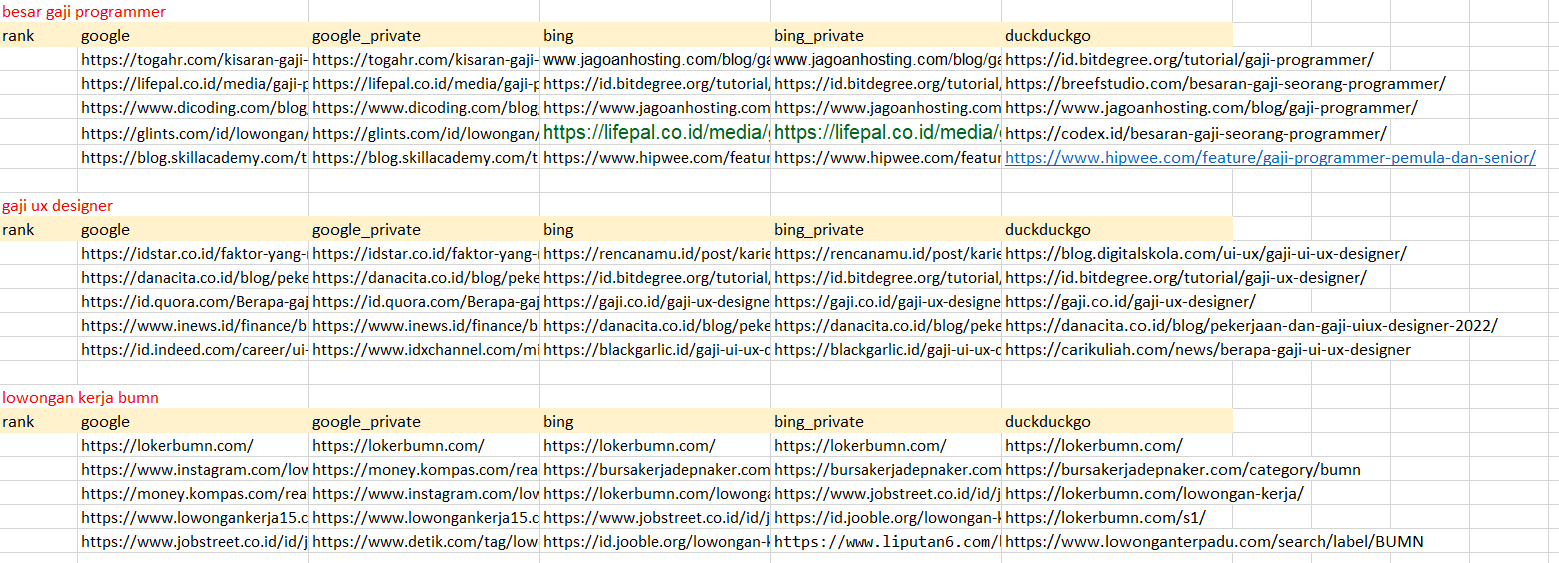
\includegraphics[keepaspectratio, width=13cm]{gambar/gambar-1002.png}
%	\caption{Contoh data yang didapat dari salah satu responden}
%	\label{gambar:gambar-1002.png}
%\end{figure}
%
%
%Setelah eksperimen selesai, dilakukan rekap hasil untuk mendapatkan hasil yang diinginkan yaitu apakah sebuah search engine melakukan personalisasi pencarian dan mengukur relevansi pencarian dari search engine.
%
%Untuk melakukan pengukuran relevansi pencarian, instruktur meminta responden untuk melakukan perangkingan dari situs situs unik yang telah dikumpulkan dari semua search engine dengan query tertentu seperti gambar berikut:
%
%%\begin{figure}[H]
%%	\centering
%%	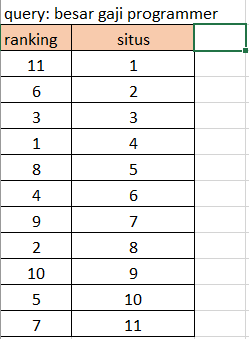
\includegraphics[keepaspectratio, width=13cm]{gambar/gambar-1003.png}
%%	\caption{Ranking situs menurut pengguna}
%%	\label{gambar:gambar-1003.png}
%%\end{figure}
%
%
%\begin{table}[H]
%	\centering
%	\caption{Ranking situs menurut pengguna}
%	\label{besar-gaji-programmer-table-result}
%	\begin{tabular}{@{}|p{4cm}|p{4cm}|@{}}
	%		\multicolumn{2}{c}{\textbf{Kata Kunci Besar Gaji Programmer}} \\
	%		\hline
	%		Ranking (rank) & Situs (site id) \\
	%		\hline
	%		11 & 1 \\
	%		\hline
	%		6 & 2 \\
	%		\hline
	%		3 & 3 \\
	%		\hline
	%		1 & 4 \\
	%		\hline
	%		8 & 5 \\
	%		\hline
	%		4 & 6 \\
	%		\hline
	%		9 & 7 \\
	%		\hline
	%		2 & 8 \\
	%		\hline
	%		10 & 9 \\
	%		\hline
	%		5 & 10 \\
	%		\hline
	%		7 & 11 \\
	%		\hline
	%		
	%		
	%	\end{tabular}
%\end{table}
%
%Untuk mengukur relevansi pencarian dari search engine, instruktur melakukan perbandingan ranking yang diberikan oleh user dengan rangking aktual dari \textit{search engine}. Untuk setiap situs dicatat selisih perbedaannya antara ranking aktual dari search enginenya dengan ranking dari user. Untuk perhitungan skor relevansi pencariannya adalah dengan cara
%\[
%Skor Relevansi = \frac{Total Selisih}{Total Selisih Yang Mungkin}
%\]
%Untuk skor lebih besar dari 0.5 maka search engine tersebut menghasilkan hasil pencarian yang tidak relevan dikarenakan selisih antara ranking aktual dan ranking pengguna terlalu besar. Untuk <= 0.5 maka hasil dari search engine dapat dibilang relevan karena memiliki selisih yang kecil. Pada proses ini setiap situs diberikan \textit{id} numerik yang unik.
%
%%\begin{figure}[H]
%%	\centering
%%	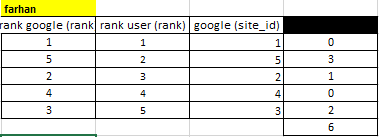
\includegraphics[keepaspectratio, width=13cm]{gambar/g-12.png}
%%	\caption{Selisih ranking dari \textit{search engine} dengan ranking pengguna}
%%	\label{gambar:g-12.png}
%%\end{figure}
%
%\begin{table}[H]
%	\centering
%	\caption{Selisih ranking dari \textit{search engine} dengan ranking pengguna}
%	\label{result-diff-2}
%	\begin{tabular}{@{}|p{3.5cm}|p{3.5cm}|p{3.5cm}|p{2cm}|@{}}
	%		\multicolumn{4}{c}{\textbf{Farhan}} \\
	%		\hline
	%		\textbf{Rank Google (rank)} & \textbf{Rank User (rank)} & \textbf{Google (site id)} & \textbf{Skor}\\ 
	%		\hline
	%		1 & 1 & 1 & 0 \\
	%		\hline
	%		5 & 2 & 5 & 3 \\
	%		\hline
	%		2 & 3 & 2 & 1 \\
	%		\hline
	%		4 & 4 & 4 & 0 \\
	%		\hline
	%		3 & 5 & 3 & 2 \\
	%		\hline
	%		\multicolumn{2}{c}{} & \multicolumn{1}{c}{Total} &  \multicolumn{1}{c}{6} \\
	%		
	%		
	%	\end{tabular}
%\end{table}
%
%
%Dari hasil penelitian yang telah dilakukan, didapatkan bahwa search engine Google memiliki skor relevansi sebesar 0.5834. Dengan skor tersebut menempatkan mesin pencari Google kedalam kategori tidak relevan sedangkan untuk mesin pencari DuckDuckGo mendapatkan skor 0.5 yang menempatkan mesin pencari DuckDuckGo ke dalam mesin pencari yang relevan.
%
%Cara mengukur personalisasi pencarian dari suatu \textit{search engine} untuk satu kata pencarian adalah dengan cara melihat perbedaan dari lima situs teratas yang disajikan. Untuk setiap ranking pencarian dilakukan perhitungan skor perbedaan, jika dua user mendapatkan situs yang berbeda pada suatu ranking maka akan mendapat skor 1 dan jika tiga user memiliki situs yang disajikan pada suatu ranking berbeda maka akan mendapat skor 2 seperti gambar dibawah berikut.
%
%
%%\begin{figure}[H]
%%	\centering
%%	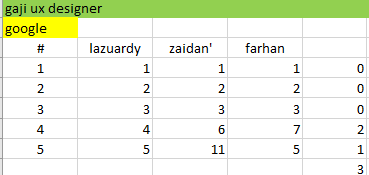
\includegraphics[keepaspectratio, width=13cm]{gambar/g-116.png}
%%	\caption{Perbedaan situs yang disajikan oleh 3 \textit{search engine} kepada 3 responden untuk kata pencarian besar gaji programmer}
%%	\label{gambar:g-116.png}
%%\end{figure}
%
%
%\begin{table}[H]
%	\caption{Perbedaan situs yang disajikan oleh 3 \textit{search engine} kepada 3 responden untuk kata pencarian besar gaji programmer}
%	\label{result-diff-1}
%	\begin{tabular}{@{}|p{0.5cm}|p{3cm}|p{3cm}|p{3cm}|p{3cm}|@{}}
	%		\multicolumn{5}{c}{\textbf{Gaji UX \textit{Designer} (Google)}} \\
	%		\hline
	%		\textbf{No.} & \textbf{lazuardy} & \textbf{zaidan} & \textbf{farhan} & \textbf{skor} \\ 
	%		\hline
	%		1 & 1 & 1 & 1 & 0 \\
	%		\hline
	%		2 & 2 & 2 & 2 & 0 \\
	%		\hline
	%		3 & 3 & 3 & 3 & 0 \\
	%		\hline
	%		4 & 4 & 6 & 7 & 2 \\
	%		\hline
	%		5 & 5 & 11 & 5 & 1 \\
	%		\hline
	%		\multicolumn{3}{c}{} & \multicolumn{1}{c}{Total} &  \multicolumn{1}{c}{3} \\
	%		
	%		
	%	\end{tabular}
%\end{table}
%
%Untuk perhitungan skor relevansi adalah sebagai berikut. Untuk skor dengan besar kurang lebih dari 5 menandakan \textit{search engine} tersebut tidak melakukan personalisasi untuk lebih dari 5 sebaliknya.
%
%\[
%Skor Personalisasi = \frac{Total Skor}{Total Skor Yang Mungkin}
%\]
%
%Cara ini digunakan untuk menguji 3 \textit{search engine} yaitu Google (Keadaan login dan tidak login), Bing (keadaan login dan tidak login) dan DuckDuckGo dan 3 kalimat pencarian. Hasil yang didapat dari masing masing \textit{search engine} adalah sebagai berikut: Google memiliki skor personalisasi sebesar 0.133 yang menandakan \textit{search engine} tersebut tidak melakukan personalisasi. Duckduckgo mendapat skor personalisasi sebesar 0.1667 yang menandakan \textit{search engine} tersebut tidak melakukan personalisasi. Bing mendapatkan skor sebesar 0.267 yang menandakan \textit{search engine} tersebut tidak melakukan personalisasi pencarian, Google dalam keadaan tidak login memiliki skor relevansi sebesar 0 yang menandakan \textit{search engine} ini tidak melakukan personalisasi pencarian dan Bing dalam keadaan tidak login memiliki skor personalisasi sebesar 0.5 yang menandakan \textit{search engine} ini tidak melakukan personalisasi pencarian.

